\documentclass[11pt]{article}
\usepackage[margin=1.1in]{geometry}
\usepackage{amsmath,amssymb,amsthm}
\usepackage[sc]{mathpazo}
\usepackage[no-math]{fontspec}
\setmainfont{TeX Gyre Pagella}
\usepackage{booktabs,array,tabularx}
\usepackage{graphicx}
\usepackage[section]{placeins}
\usepackage[font=small,labelfont=bf]{caption}
\usepackage{microtype}
\usepackage[hidelinks]{hyperref}
\usepackage{tikz}
\usetikzlibrary{arrows.meta,positioning}

\newtheorem{definition}{Definition}
\newtheorem{proposition}{Proposition}
\newtheorem{corollary}{Corollary}
\theoremstyle{remark}
\newtheorem{remark}{Remark}

\setlength{\parskip}{0.35em}
\renewcommand{\arraystretch}{1.15}

\title{Cutaway Reader\\[0.4em]
\large Spatial Memory, Append-Only Place, and the Navigation of a Written Corpus}
\author{Flyxion\\ \small Independent Researcher}
\date{September 2026}

\begin{document}
\maketitle

\begin{abstract}
A corpus of several hundred essays and books, written as linear LaTeX documents, is usually approached through search: a query returns a list, the list returns a page, and nothing about the route survives the visit. This essay describes the Cutaway Reader, a working system that compiles each work into a small navigable level and places the works of a corpus in a galaxy, so that a reader acquires place memory of an argument in the way a player acquires the topology of a well-designed mine. Sections become chambers and subsections alcoves; references become tunnels that are physically two-way and semantically directed; appendices descend as a shaft; and the directions of space carry fixed meanings, with foundations below, consequences above, comparisons to the side, and the main passage forward. The design takes two games of 1995 as its reference points: \emph{Descent}, for continuous six-degree-of-freedom navigation paired with a rotatable cutaway automap, and \emph{Stars!}, for supervisory control through routes and policies. Its central engineering commitment is a separation between meaning, recomputed from the sources on every build, and place, kept in an append-only ledger so that revision can enlarge a level but never rearrange what a reader has learned. A second commitment treats every reading action as an event in a replicated log whose state is derived by replay, so that the cockpit, the automap, a text navigator and a terminal client are views of one history. The essay sets out the motivations, the mapping from document to level, the verbs available to a reader, the log and its merge semantics, the corpus layer with its placement ledger and typed lanes, the implementation and its testing discipline, and a first trial on ten real works totalling about 122,000 words. It then gives mathematical interpretations of the main structures (append-only embeddings as monotone partial maps, reader state as a fold over a join-semilattice, placement as constrained stress minimisation with deliberate path dependence, semantic zoom as a tower of quotients, and on-demand loading as a factorisation through an index) and relates the system to earlier work on event-history computation, layered persistent worlds, recoverable distinction, source-first publishing, and reachability. It closes with what the system has not yet shown, beginning with the untested claim on which the whole design rests: that a reader who closes it will remember where an argument was.
\end{abstract}

\newpage

\section{Introduction}
\label{sec:intro}

A written corpus of any size develops a characteristic failure of orientation. Each work is internally ordered, but the relations between works, and even the large-scale shape of a single long argument, are carried only in the author's memory and in scattered cross-references. A reader arriving from a search engine lands in the middle of a text with no sense of what lies above, below or beside the paragraph in view. Returning a week later, the same reader finds nothing that records how the passage was reached or what was nearby. Retrieval succeeds and orientation fails. The failure is not a defect of search, which does what it is built to do, but a consequence of treating a corpus as a set of addressable pages rather than as a space that can be learned.

The Cutaway Reader begins from the observation that some interactive environments are remarkably good at producing durable spatial knowledge of structures far more confusing than a book. The mines of \emph{Descent} \cite{descent} are enclosed three-dimensional tunnel systems in which floor and ceiling are conventions the player can abandon at will, yet players routinely come to know them well enough to plan escapes under pressure. That knowledge does not come from a map handed over at the start. It comes from traversal, from return, from partial revelation, and from a second representation, the cutaway automap, that strips away texture and lighting to preserve connectivity and can be rotated until it agrees with the player's internal sense of the level. The map is a severe abstraction that supports recollection. It does not claim to be the world.

The proposal is to give each work in a corpus that kind of structure. A LaTeX source is compiled into a level whose chambers are its sections and whose tunnels are its references. The reader flies through it with continuous six-degree-of-freedom controls, opens the cutaway map to see the explored topology, and reads the prose at a fixed reading station in the ordinary vertical manner. Above the individual levels sits a supervisory layer modelled on \emph{Stars!} \cite{stars}, in which works are systems in a galaxy, lanes join them, and a reader can declare routes and policies and let a cruise carry them through a sequence of chambers. The text itself is never distorted into walls or scattered across a scene. The spatial interface surrounds reading without replacing it.

Two constraints turn this from a visual metaphor into a system. The first is stability. If revising an essay regenerated its level from scratch, every edit would reshuffle the chambers and destroy exactly the place memory the design exists to produce. The Cutaway Reader therefore separates meaning from place. Meaning, in the narrow sense of the graph of what connects to what, is recomputed from the sources on every build. Place, the position of each chamber and each work, is written once into an append-only ledger and never moved. Revision can dig new chambers and seal withdrawn ones; it cannot rearrange the learned mine. The second constraint is honesty about what was inferred. The system infers roles from headings, lanes from citations, and a proposed edition when a work exists in several drafts, and each inference is marked as such until a person decides. A lane guessed from prose is never drawn at all; it is listed as a suggestion.

The system exists as working software: a LaTeX miner, a corpus builder with an import pipeline, a shared JavaScript model, a WebGL cockpit with touch controls, a text navigator and a terminal client, together with schemas for every file format and just over a hundred automated checks. It has been run on a first trial of ten real works, including two long monographs, and the trial exposed both parser failures and properties of the corpus that were not visible before, such as works that share subject matter but have no declared connection. The sections that follow describe the design in the order in which its commitments constrain one another: the reference designs and the psychology of place (Sections~\ref{sec:loops} and~\ref{sec:place-memory}), the compilation of a work into a level (Section~\ref{sec:level}), the append-only ledger (Section~\ref{sec:ledger}), the reader's verbs (Section~\ref{sec:verbs}), the event log (Section~\ref{sec:log}), the corpus layer (Section~\ref{sec:corpus}), the implementation (Section~\ref{sec:impl}), the trial (Section~\ref{sec:trial}), mathematical interpretations (Section~\ref{sec:math}), connections to related frameworks (Section~\ref{sec:connections}), and limits (Section~\ref{sec:limits}).

\section{Two Loops: Descent and Stars!}
\label{sec:loops}

The design takes two games as its reference points, and the choice is structural rather than nostalgic. Each supplies one of two distinct cognitive loops that the reader is meant to run.

\emph{Descent} supplies an embodied local loop. The player occupies a position inside an enclosed topology and moves through it continuously. Six degrees of freedom are available at once: three translations (surge, strafe, heave) and three rotations (pitch, yaw, roll). No movement mode has to be selected before a compound motion can be performed; a player can thrust forward, strafe, rise, pitch and roll in a single gesture, so that the route through a tunnel is remembered partly as a motor sequence. The control layout adopted here keeps that property and assigns it to two hands in a way that follows the spatial grammar of the Vim editor: the right hand orients with H, J, K and L for yaw and pitch, the left hand translates with W and S for thrust, A and D for strafe, and R and F for vertical motion, and Q and E roll. The keys never change meaning in flight. W is always forward motion and never ``next essay'', because once a key stands for a document operation the embodied coherence disappears and the environment becomes a slideshow operated from the keyboard.

The cutaway automap in \emph{Descent} is a second perception-and-control loop layered over the first. The local loop concerns the wall, the doorway, the corridor ahead. The map loop concerns cycles, shortcuts, escape routes and reachability. It opens in the player's current orientation, can be rotated with the same controls used for flight, and shows only what has been explored, with doors and objects in sparse colour against a white skeleton. Late levels of the game also show the map's failure mode: when every edge of a large mine is displayed at once the wireframe becomes a thicket, and the map remains useful only because the player has already acquired the space by moving through it. The lesson taken here is that a map for a corpus must be egocentric before it is exhaustive, local before it is global, and must change representation, not merely scale, as it widens.

\emph{Stars!} supplies a supervisory loop. It is a turn-based strategy game of galactic expansion in which the player's work is largely the declaration of standing arrangements: repeating freighter routes, patrol boundaries, production queues, and policies that govern behaviour within bounds. After enough infrastructure is in place, the player can advance turns while trusting it. The progression that matters is from direct control to a repeatable route, from a route to a bounded policy, and from a policy to supervisory trust. The game also preserves state across absence. A player returning after several days does not face an undifferentiated mass of planets but a record of where things stood, which routes were active and what changed. For a reader of a large corpus, resumability of this kind is more valuable than any conventional reward.

The two loops are not competing interfaces. They expose different temporal and spatial scales of one state. The Cutaway Reader keeps their visual grammars distinct for that reason: the local mode is a green wireframe cockpit with a rotatable cutaway map, while the supervisory mode is sparse, largely textual and information-dense. Rendering an entire corpus as one enormous three-dimensional universe would reproduce the thicket at a grander scale. The strategic screen summarises, the tunnel situates, and the reading screen disappears into the text.

The synthesis has a history in earlier projects that pursued parts of it separately. Haplopraxis, a game-scale design from around 2023, already combined the strategic persistence of \emph{Stars!} with the embodied exploration of \emph{Descent}, typing-tutor mechanics and simulation, but as a game and educational environment rather than an interface to writing. Polyxan moved the subject toward knowledge organisation: papers, simulations and media with provenance, typed links and non-file versioning, and a reading of the docuverse of Nelson's Project Xanadu, whose file structure for linked and versioned text was first proposed in 1965 \cite{nelson1965}, as a semantic plenum through which readers define their own trajectories. Later work projected embeddings into a three-dimensional starspace with finite travel times, per-reader local frames and append-only history, and treated navigation explicitly as reasoning, territory as committed history, and local action as change that propagates into a strategic layer. The essay ``Trajectories All the Way Down'' supplied the bridge from flight to thought in a formulation that can stand as the epigraph of the present design: the player does not compute a path, but applies simple local controls that accumulate into whatever trajectory the task requires, so that inference is navigation rather than lookup. What is new in the Cutaway Reader is the specific editorial and generative synthesis: each LaTeX work compiled deterministically into one level, the fixed semantic axes, the reinterpretation of the game's spare verbs as reading operations, and the rule that revision may enlarge a mine but must never destroy its learned topology.

\section{Memory for Places}
\label{sec:place-memory}

The claim that spatial structure aids the memory of arguments has a long history and a substantial experimental literature, and both deserve a careful statement because the design stakes a great deal on them.

The classical art of memory placed the items to be remembered at loci in an imagined building and recalled them by walking its rooms \cite{yates1966}. The method works because spatial sequence is easier to retain than arbitrary sequence and because each locus is distinct. Experimental psychology later gave the underlying capacity a name. Tolman's studies of rats in mazes argued that animals acquire a cognitive map, a representation of the layout of an environment that supports novel shortcuts rather than merely a chain of learned responses \cite{tolman1948}, and O'Keefe and Nadel located a neural substrate for such maps in the hippocampus \cite{okeefe1978}. Studies of how people learn large environments describe a progression from landmarks to routes between landmarks to survey knowledge of the configuration as a whole \cite{siegel1975}. Lynch's study of how inhabitants picture their cities identified the elements that make an environment imageable: paths, edges, districts, nodes and landmarks \cite{lynch1960}. A level of the Cutaway Reader is built to supply each of these deliberately. The main passage is a path; the boundary of a part is an edge; a series of works is a district; junction chambers where references converge are nodes; and chambers distinguished by an illustration, a thesis marker or an open thread are landmarks.

Work on navigation in virtual environments is more cautious and more directly relevant. Darken and Sibert found that people in large virtual worlds become disoriented without structural cues and benefit from organising principles such as paths and landmarks \cite{darken1996}. Ruddle, Payne and Jones found that people who navigated desktop virtual buildings over extended practice came to acquire spatial knowledge comparable in several respects to that acquired in real buildings \cite{ruddle1997}. In document management specifically, Robertson and colleagues showed that people who had arranged thumbnails of web pages themselves on an inclined plane that exploited spatial memory retrieved them faster than with a conventional list of bookmarks \cite{robertson1998}. None of these results shows that a three-dimensional level makes an argument memorable. They show that spatial memory is a real resource, that it forms through traversal and arrangement, and that it is fragile when structure is absent or when the arrangement changes under the user. The last point is the one the Cutaway Reader's ledger is built around.

The contrast case that motivated the design is instructive. A large archive of a computing magazine rendered as a zoomable mosaic of page thumbnails preserves every page faithfully while losing nearly every useful relationship; zooming enlarges the field without changing what kind of thing is shown, and the result is exhaustive fidelity that produces noise. Two principles follow from the comparison. The first is that a memorable interface changes representation between scales. At the widest scale it shows regions and connections, at an intermediate scale recognisable landmarks and routes, and at close range the objects themselves. This is semantic zoom in the sense of the zoomable interfaces of Perlin and Fox and of Bederson and Hollan \cite{perlin1993,bederson1994}, and it differs from the familiar maxim of information visualisation, overview first, then zoom and filter, then details on demand \cite{shneiderman1996}, in one respect that matters: the automap opens egocentrically, centred on the reader, and becomes exhaustive only on request. A local map with seven recognisable connections is more navigable than a truthful picture of six hundred works. Furnas's generalised fisheye views give the same principle a formal shape, weighting what is shown by a priori importance and distance from the focus \cite{furnas1986}.

The second principle is that movement must have consequences. If every point can be reached instantly from a search result, the user may retrieve information without acquiring a place. In \emph{Descent}, finding a key changes which doors are passable, opening a shortcut revises the topology, and revisiting a chamber reveals it from another orientation. The Cutaway Reader adopts milder equivalents. Travel through a level follows real passages and is recorded; a jump between works follows a lane and is recorded as a jump; arriving without a lane, from the galaxy or a search, is permitted but recorded honestly as a warp and counted separately. Orientation, in the end, comes from invariants amid transformation. A player may roll upside down and approach a chamber along another axis, yet its connections stay the same. An interface that allows filtering, zooming and revision while keeping enough structure fixed that the user knows what changed and what did not is one in which memory can accumulate.

Illustrations enter the design under the same principle. In old magazines and comics, advertisements interrupt the narrative every few pages and force the reader to rebuild its atmosphere on each return. The rule adopted for the corpus is the opposite: an illustration sits at the head of a section, where comprehension naturally resets, and is followed by uninterrupted prose until the next section boundary, so that the image prepares continuity rather than competing with it. On the automap such an image becomes a landmark glyph, and a reader who cannot recall a subsection's title may still recall the chamber beneath a particular picture. Illustration landmarks are specified but not yet generated for the trial corpus; Section~\ref{sec:limits} returns to them.

\section{A Work as a Level}
\label{sec:level}

The unit of compilation is one work: a LaTeX source together with every file it reads through \texttt{\textbackslash input}, \texttt{\textbackslash include} and a named bibliography database. The miner reads the source as it is written, without requiring any change to it, and produces two artifacts: a graph describing what the work contains and how its parts connect, and a ledger describing where each part sits in space. This section describes the graph. The ledger is the subject of Section~\ref{sec:ledger}.

\subsection{Chambers, alcoves and passages}

The document's own top level of sectioning becomes a chamber and the level below it an alcove. In an article, \texttt{\textbackslash section} is a chamber and \texttt{\textbackslash subsection} an alcove; in a book, where \texttt{\textbackslash chapter} carries the argument, a chapter is a chamber and a section an alcove. Deeper headings do not become space. They remain in the chamber's text as marked lines, because geometry belongs only at the scale where it affects the next navigational decision, and a level with a room for every paragraph heading would be the thicket the automap is meant to avoid. \texttt{\textbackslash part} groups chambers on the map without becoming a chamber itself, and the miner advises splitting any part that holds more than twenty chambers. Starred back matter (bibliography, references, index) is not dug at all.

Passages come in five kinds, summarised in Table~\ref{tab:mapping}. The sequence passage joins the chambers of the main passage in reading order. A chamber that is not on the main passage, such as a foundation, a consequence or a comparison, is joined by a branch to the main chamber it follows, so that the reading passage itself remains a clear line and does not detour through side chambers. Appendices hang from the last main chamber as a descending shaft. Each alcove opens from its parent chamber. Finally, every \texttt{\textbackslash ref} from one chamber to a label in another becomes a reference tunnel. When the referenced chamber is a foundation, the tunnel carries a door, marking a prerequisite: the passage is open, but the map shows that the chamber on the far side is something the present one rests on.

\begin{table}[htbp]
\centering\small
\begin{tabularx}{\linewidth}{>{\raggedright}p{0.33\linewidth}X}
\toprule
In the source & In the level \\
\midrule
top-level section (\texttt{\textbackslash section}, or \texttt{\textbackslash chapter} in a book) & a chamber, sized by its word count \\
next level down & an alcove opening from its chamber, kept level with it \\
deeper headings & a marked line in the chamber's text \\
consecutive main sections & a sequence passage, forward in reading order \\
a section off the main passage & a branch from the main chamber it follows \\
appendices & a shaft descending from the last main chamber \\
\texttt{\textbackslash ref} to another chamber & a reference tunnel, physically two-way, directed from citing to cited \\
\texttt{\textbackslash ref} to a foundation & the same tunnel with a door (a prerequisite) \\
\texttt{\% mine: exit=work\#label} & a portal to another work, two-way \\
\texttt{\% mine: continue=work} & a portal that is one-way, reserved for real irreversibility \\
\texttt{\% thread[kind]: text}, \texttt{\textbackslash todo} & an open thread marked in the chamber \\
display mathematics & an \emph{[equation]} marker that keeps its labels \\
\bottomrule
\end{tabularx}
\caption{The mapping from a LaTeX source to a level.}
\label{tab:mapping}
\end{table}

Reference tunnels are physically two-way and semantically directed. A reader can always fly back through a tunnel, because a one-way passage in an explored space is a trap that punishes curiosity. The tunnel nevertheless remembers which chamber cited which, and the passage list describes it from each end accordingly, as a tunnel to a section cited here or a tunnel back to a section that cites this one. One-way passages exist only where the author declares a real irreversibility, through a \texttt{continue=} directive, and then only between works.

\subsection{Fixed axes}

Directions carry the same meaning in every work, so that a reader's sense of orientation transfers from one level to the next. The main passage runs forward along the positive $z$ axis. Foundations lie below it, consequences above it, comparisons to one side along $x$, and appendices descend in a shaft. Alcoves stay in the horizontal plane of their parent chamber, spread at fixed angles, so that they never read as foundations or consequences. The result is that a vertical movement always means the same kind of relation. Descending is moving toward what an argument rests on; rising is moving toward what it opens. A reader who has learned that in one essay has learned it for all of them.

The role of a chamber is taken from an explicit directive when the author supplies one (\texttt{\% mine: role=foundation}, for instance) and is otherwise inferred from its heading: headings mentioning preliminaries, definitions, background, notation, axioms or a framework are read as foundations; applications, extensions, implications and outlook as consequences; objections, comparisons, contrasts, alternatives and replies as comparisons; everything else as the main passage. The inference is deliberately crude and deliberately visible. The passage list names the role of every chamber in axis words (``down to foundation'', ``up to consequence'', ``side passage to comparison'', ``back up to the main passage'', ``down the appendix shaft''), so a wrong inference is obvious the moment a reader meets it, and one line of source corrects it.

\subsection{Directives, threads and portals}

The author speaks to the miner through LaTeX comments, so every source still compiles unchanged. \texttt{\% mine: thesis} marks the chamber that carries the central claim; \texttt{\% mine: role=} fixes a role; \texttt{\% mine: exit=} declares a portal to another work, optionally to a labelled chamber in it; and \texttt{\% mine: continue=} declares a one-way portal. Open threads are declared as \texttt{\% thread[kind]: text}, and a \texttt{\textbackslash todo} becomes a thread of kind \emph{missing}.

Threads have four kinds: \emph{missing} work, an optional \emph{extension}, unresolved \emph{evidence}, and principled \emph{openness}, a question left open on purpose. The design borrows their place in the level from the hostages of \emph{Descent}, who are found in particular rooms and give the player a reason to explore off the main route, but it refuses the game's rescue score. Threads are marked, not graded. A corpus in which every open question counted against a total would reward closing questions for the sake of the count, and some questions ought to stay open.

\subsection{Reading text}

Each chamber carries the prose of its section as plain reading text, prepared for a reading station rather than for print. The miner expands the author's zero-argument macros, turns theorem environments into their names (``Proposition (Separation).''), renders inline mathematics legibly with Greek letters and common symbols, replaces each display by an \emph{[equation]} marker that keeps its labels so references to it still resolve, drops page furniture such as table-of-contents entries and spacing commands, and decodes accents and escaped characters. A section's text is shown at a fixed reading station in ordinary vertical layout; the reader does not read on the walls. The reading station exists because reading and flying need different key bindings. Inside the station the keys scroll and search; outside it they fly. The transition is explicit, and each mode preserves the other's state.

\section{Place Is Remembered}
\label{sec:ledger}

Everything in Section~\ref{sec:level} is recomputed from the sources on every build. If place were recomputed too, the level would be a pure function of the current text, and every revision would be free to move every chamber. A reader who had learned that the chamber on objections lay to the left of the third main chamber would return to find it somewhere else, or find that the third main chamber was now the fourth and stood where the second had been. Place memory cannot survive that. The central engineering decision of the Cutaway Reader is therefore to keep two artifacts per work with different change rules. The graph is recomputed. The ledger only grows.

\subsection{Digging}

The ledger records, for every chamber ever seen, its position, its radius, its role and level, its parent, whether it is active or withdrawn, and when it was first and last seen. A build walks the chambers of the current source in order. A chamber already in the ledger keeps its position; its radius may grow if its section has grown, but it never shrinks and the chamber never moves. A chamber not yet in the ledger is dug: it is placed relative to an anchor, the previous main chamber for a main or off-axis chamber, the previous appendix for an appendix, the parent for an alcove, at a standard spacing of forty units along its role's axis. If that position collides with an existing chamber, meaning that the two spheres would come closer than the sum of their radii plus a gap, the digger first tries to set the new chamber inside the existing gap on the same axis, at a half, a third or two thirds of the spacing, so that a section inserted between two others appears between them. Only then does it search outward in rings perpendicular to the axis. Chamber radii grow with the square root of the section's length and are capped, so a long section is a larger room without dominating the level.

A section that disappears from the source is not erased. Its chamber is marked withdrawn and remains in the ledger, sealed, visible on the map as a closed room and never reused for another section. The history of each build records which chambers were added, which were extended and which were withdrawn, so the panel can tell a returning reader what changed in the source since the last visit.

\subsection{Identity}

The rule that a known chamber keeps its position requires a rule for when two chambers in successive builds are the same chamber. A labelled section is identified by its label, so it survives renaming, reordering and rewriting; its identifier has the form \texttt{L:}\emph{label}. An unlabelled section is identified by its level, its parent and the slug of its heading, with an occurrence index to separate repeated headings under one parent; its identifier has the form \texttt{G:}\emph{slug}. The ledger keeps both mappings, labels to identifiers and heading keys to identifiers in order of occurrence, so identity is a matter of recorded history rather than of recomputation.

The consequence is stated plainly in the documentation and in the corpus report: renaming the heading of an unlabelled section digs a new chamber and withdraws the old one. That is not a defect to be hidden but the correct behaviour given the information available. If nothing in the source ties the renamed section to its predecessor, the system has no ground for asserting continuity, and asserting it anyway would be a guess presented as a fact. A \texttt{\textbackslash label} is the author's statement that a section persists through revision, and the ledger honours it.

\begin{proposition}[Learned topology is preserved]
\label{prop:preserved}
Let a chamber $c$ be dug at build $t_0$ with position $p$. For every later build $t \ge t_0$, the ledger records $c$ at position $p$, whether $c$ is active or withdrawn at $t$.
\end{proposition}

The proof is immediate from the construction: positions are written only when an identifier is absent from the ledger, and no operation removes an identifier. The proposition is nonetheless the one property on which the whole design depends, and it is checked directly by the test suites, which rebuild levels and galaxies and compare positions before and after. Section~\ref{sec:math} gives it an algebraic form.

\section{The Verbs of a Reader}
\label{sec:verbs}

\emph{Descent} gives the player a small set of verbs beyond movement: primary and secondary fire, flares, bombs, a rear view, and an automap. The Cutaway Reader reinterprets each as a reading operation, keeping the physical gesture and changing its object.

\subsection{Movement and reading}

The six-degree control surface described in Section~\ref{sec:loops} is available whenever the reader is in flight: W and S for thrust, A and D for strafe, R and F for vertical motion, H, J, K and L (or the arrow keys) for yaw and pitch, and Q and E for roll. Crossing from one chamber into another through a passage is recorded as a traversal followed by an entry. Enter opens the reading station for the current chamber. On a phone or tablet the same motions are driven by a joystick for translation, a drag across the view for orientation, and buttons for vertical movement; on the map, the vertical buttons change the map's depth instead, a drag rotates it, a pinch zooms, and a tap selects a system.

\subsection{Inspect, bind and beacon}

Primary fire becomes inspection (Y, or the space bar): the passage ahead is identified and its destination described before it is taken, including the destination's role and whether it is a prerequisite. Secondary fire becomes binding (U): the inspected chamber is added to a route the reader is building. A bomb becomes a beacon (B): a numbered mark dropped at the reader's exact position and orientation, with a short note, such as a reminder that a comparison with another work belongs here or that a citation is needed. A beacon remembers where it was dropped, which way the reader was facing, the last three passages traversed to reach it, and why. It appears in the level, on the automap, where the number keys find it, and in the supervisory panel. A beacon is retired, not deleted, and the retirement is itself recorded.

\subsection{Scan}

A flare becomes a scan (G). A scan reveals the layout within seventy units of the reader for twenty seconds and then fades. It shows shape, not contents: glimpsed chambers and tunnels appear on the map as outlines in a distinct state, and a scan opens no chamber's text. The limit is deliberate. Permanent knowledge comes only from being there. A scan lets a reader see whether a region is worth visiting without converting a glance into acquaintance, and the chamber states make the difference visible. A chamber is \emph{unexplored} until something reveals it; \emph{glimpsed} while a scan covers it; \emph{revealed} once a neighbouring chamber has been visited, since a visited chamber shows its own doorways; and \emph{visited} once entered. Passages have the matching states \emph{glimpsed}, \emph{revealed} and \emph{traversed}.

The vocabulary is fixed because it is shared with other work. In Haplopraxis a flare is a persistent shared inscription, an act of leaving a public mark in a world. The Cutaway Reader's first prototype called its temporary glimpse a flare, and the name was changed so that the two meanings could not be confused: here a scan is temporary, a beacon is persistent and personal, and flare is reserved and never produced. Logs written before the rename are upgraded on load, with the old name kept on the event for provenance.

\subsection{Rear view, path and cruise}

Holding O shows the optical rear view, the scene behind the reader, which in a tunnel system is the route of arrival. Holding P replays the path taken, drawing the trail through the level. These two verbs make route ancestry visible without requiring the reader to have attended to it on the way in.

Cruise is the point at which the supervisory loop enters the cockpit. A policy selects the stops of a route: \emph{reading} follows the reading order; \emph{prerequisites first} visits the foundations a chamber rests on before the chamber itself; \emph{open threads} visits the chambers with threads; and \emph{bound} follows the chambers the reader has bound. Pressing C starts the cruise, and the ship then flies the route as an actual trajectory through the tunnels, facing where it is going, with C and Z to change speed and X to stop. Any manual input takes control back. The cruise is thus not a teleport between search results but a supervised flight through real passages, in the spirit of the repeating freighter routes of \emph{Stars!}: the reader declares where to go and under what policy, and then rides the declaration. Every stop the cruise reaches is recorded exactly as a manual flight would be.

\subsection{The automap}

Tab, or the semicolon beside the orientation keys, opens the automap. A brief tap latches it open; holding it peeks and releases on key-up. The map opens centred on the reader in the reader's current orientation and rotates with the same keys used for flight. White is the architectural skeleton of traversed passages; revealed structure is blue; the reader and the recent trail are green; the active route is amber; prerequisite doors are orange; portals to other works are magenta; and open threads are red. Colour is sparse and invariant, carrying only actionable distinctions.

The map's depth changes representation rather than scale (Figure~\ref{fig:views}). At the closest depth it shows the current chamber and its neighbours. One step out shows the whole work as a chamber graph. One step further, the work collapses into a single system and the galaxy appears, with the reader's work highlighted, its lanes drawn, and other systems selectable; a second selection of the same system travels there. At each step the geometry is simplified to what can affect the next decision, so that the map never becomes a picture of everything at once.

\begin{figure}[htbp]
\centering
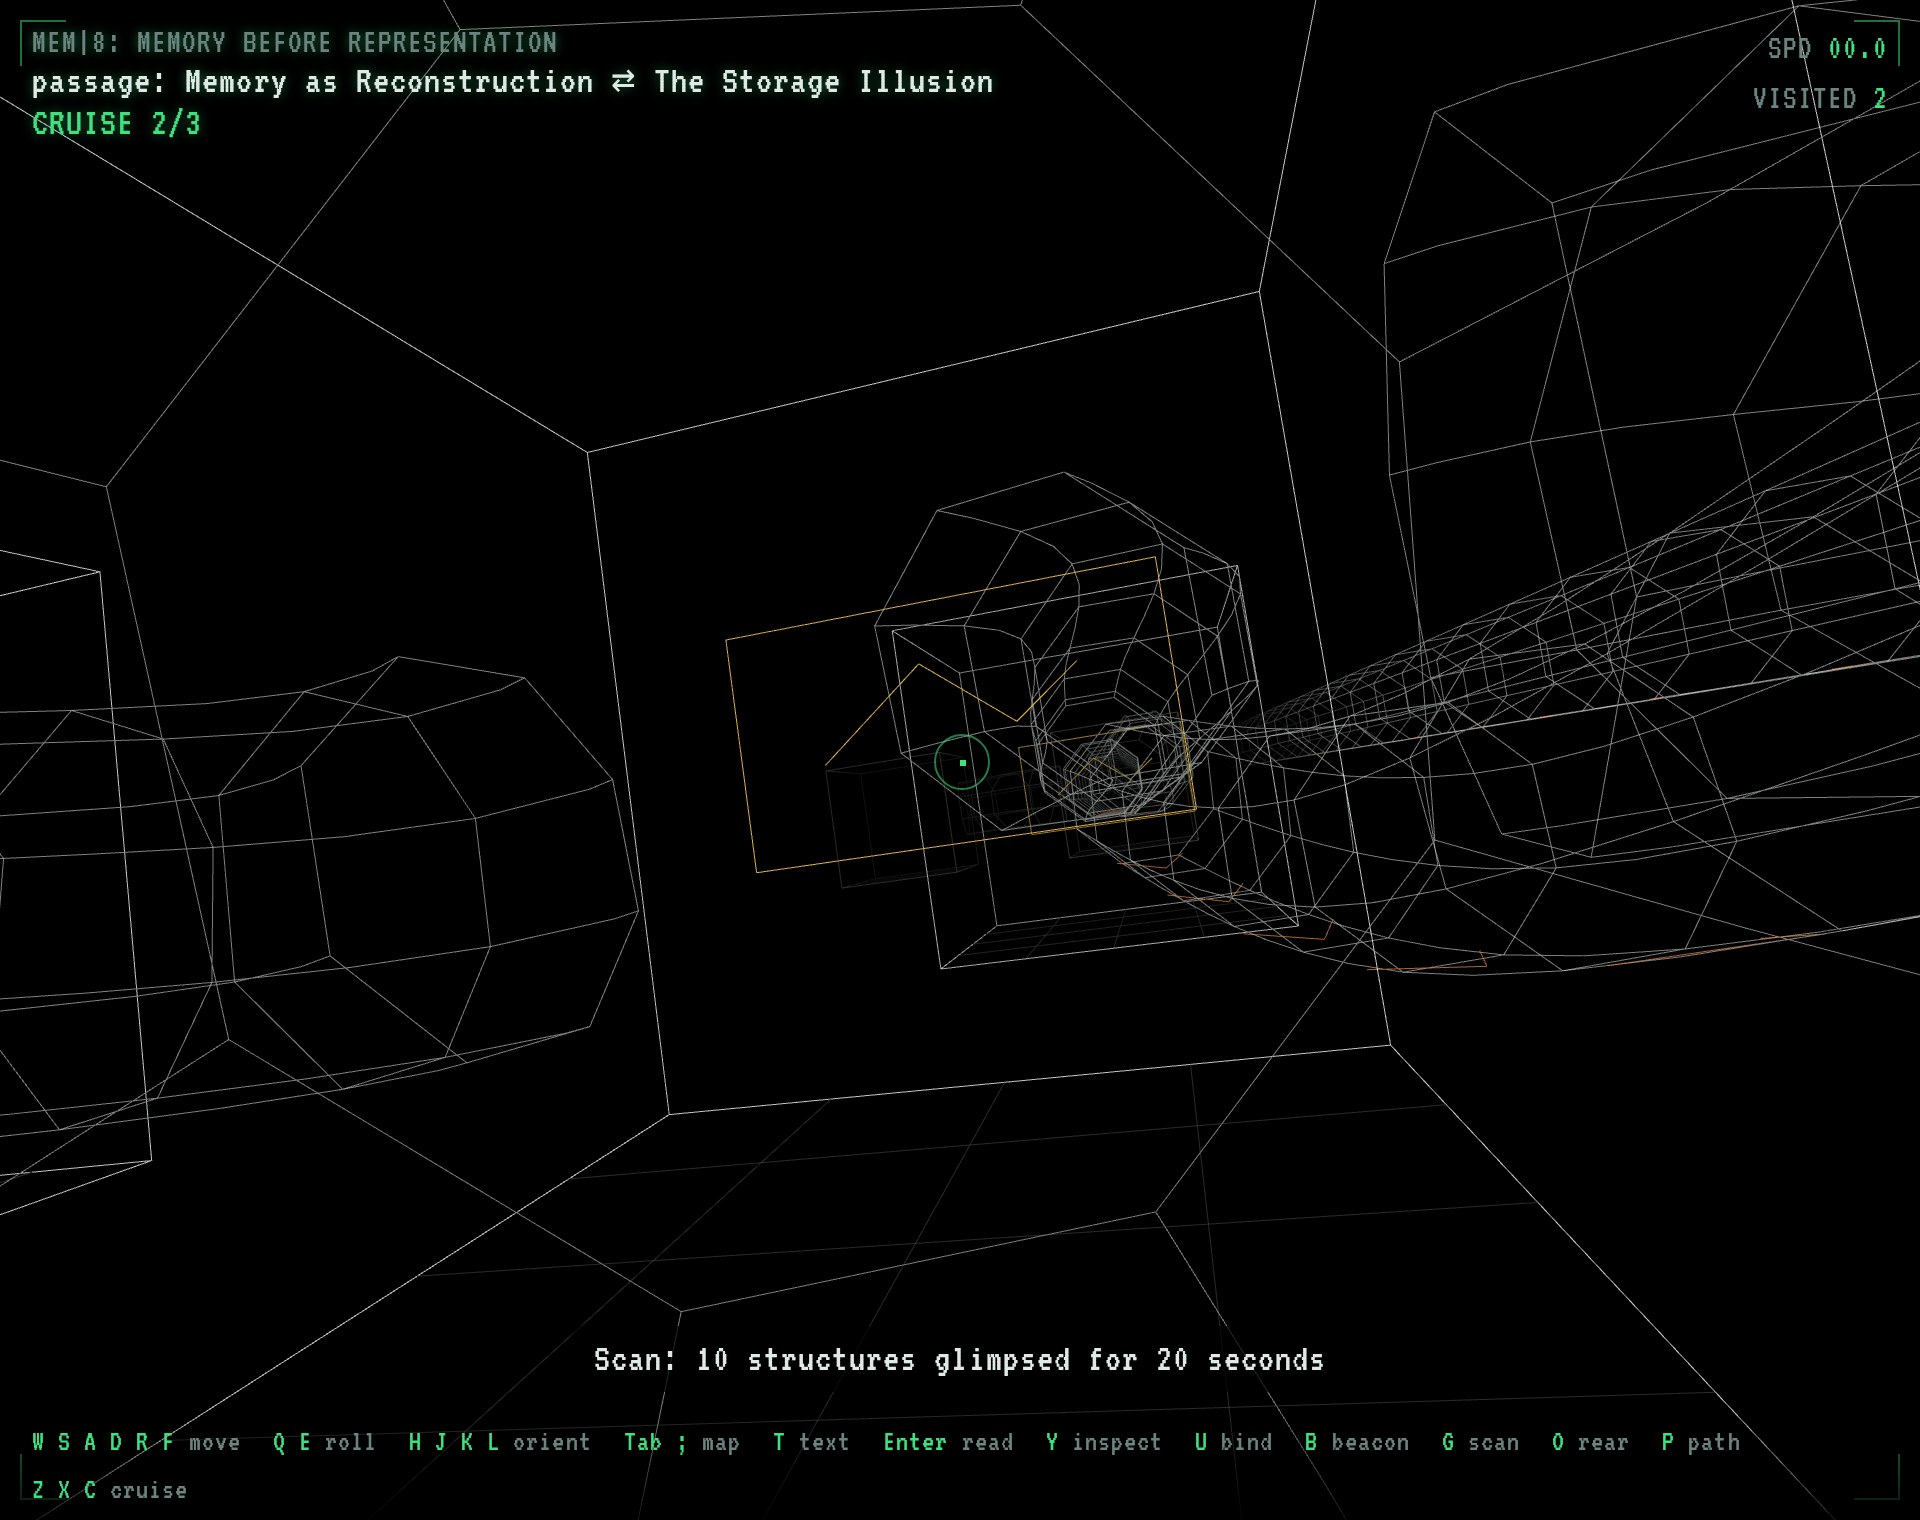
\includegraphics[width=0.49\linewidth]{fig/cockpit-crop.jpg}\hfill
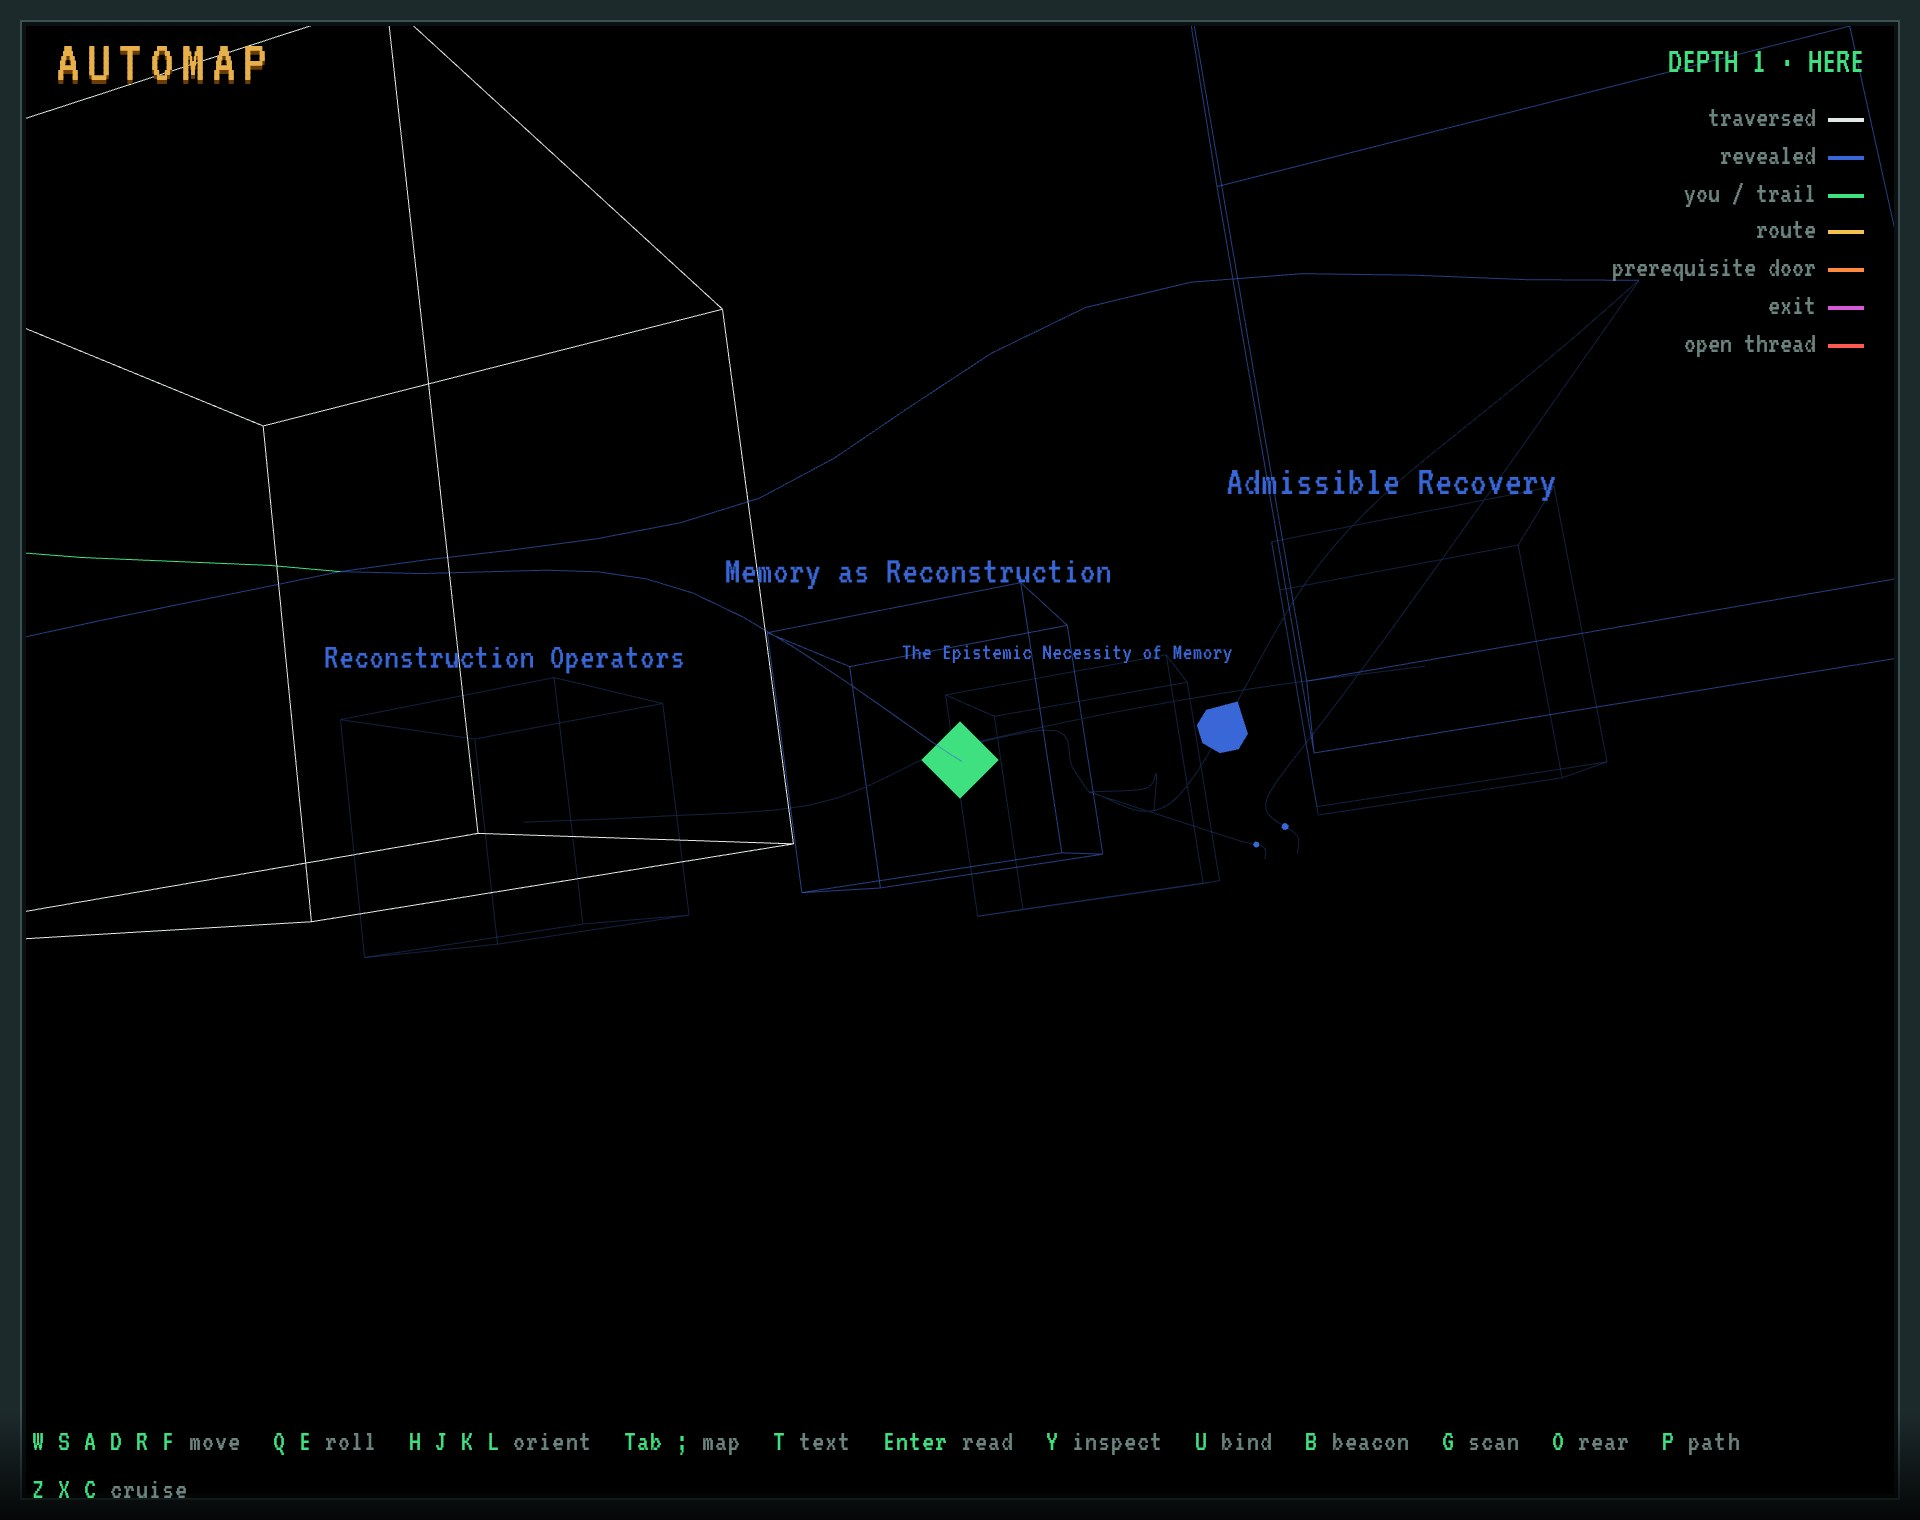
\includegraphics[width=0.49\linewidth]{fig/map-local-crop.jpg}\\[0.5em]
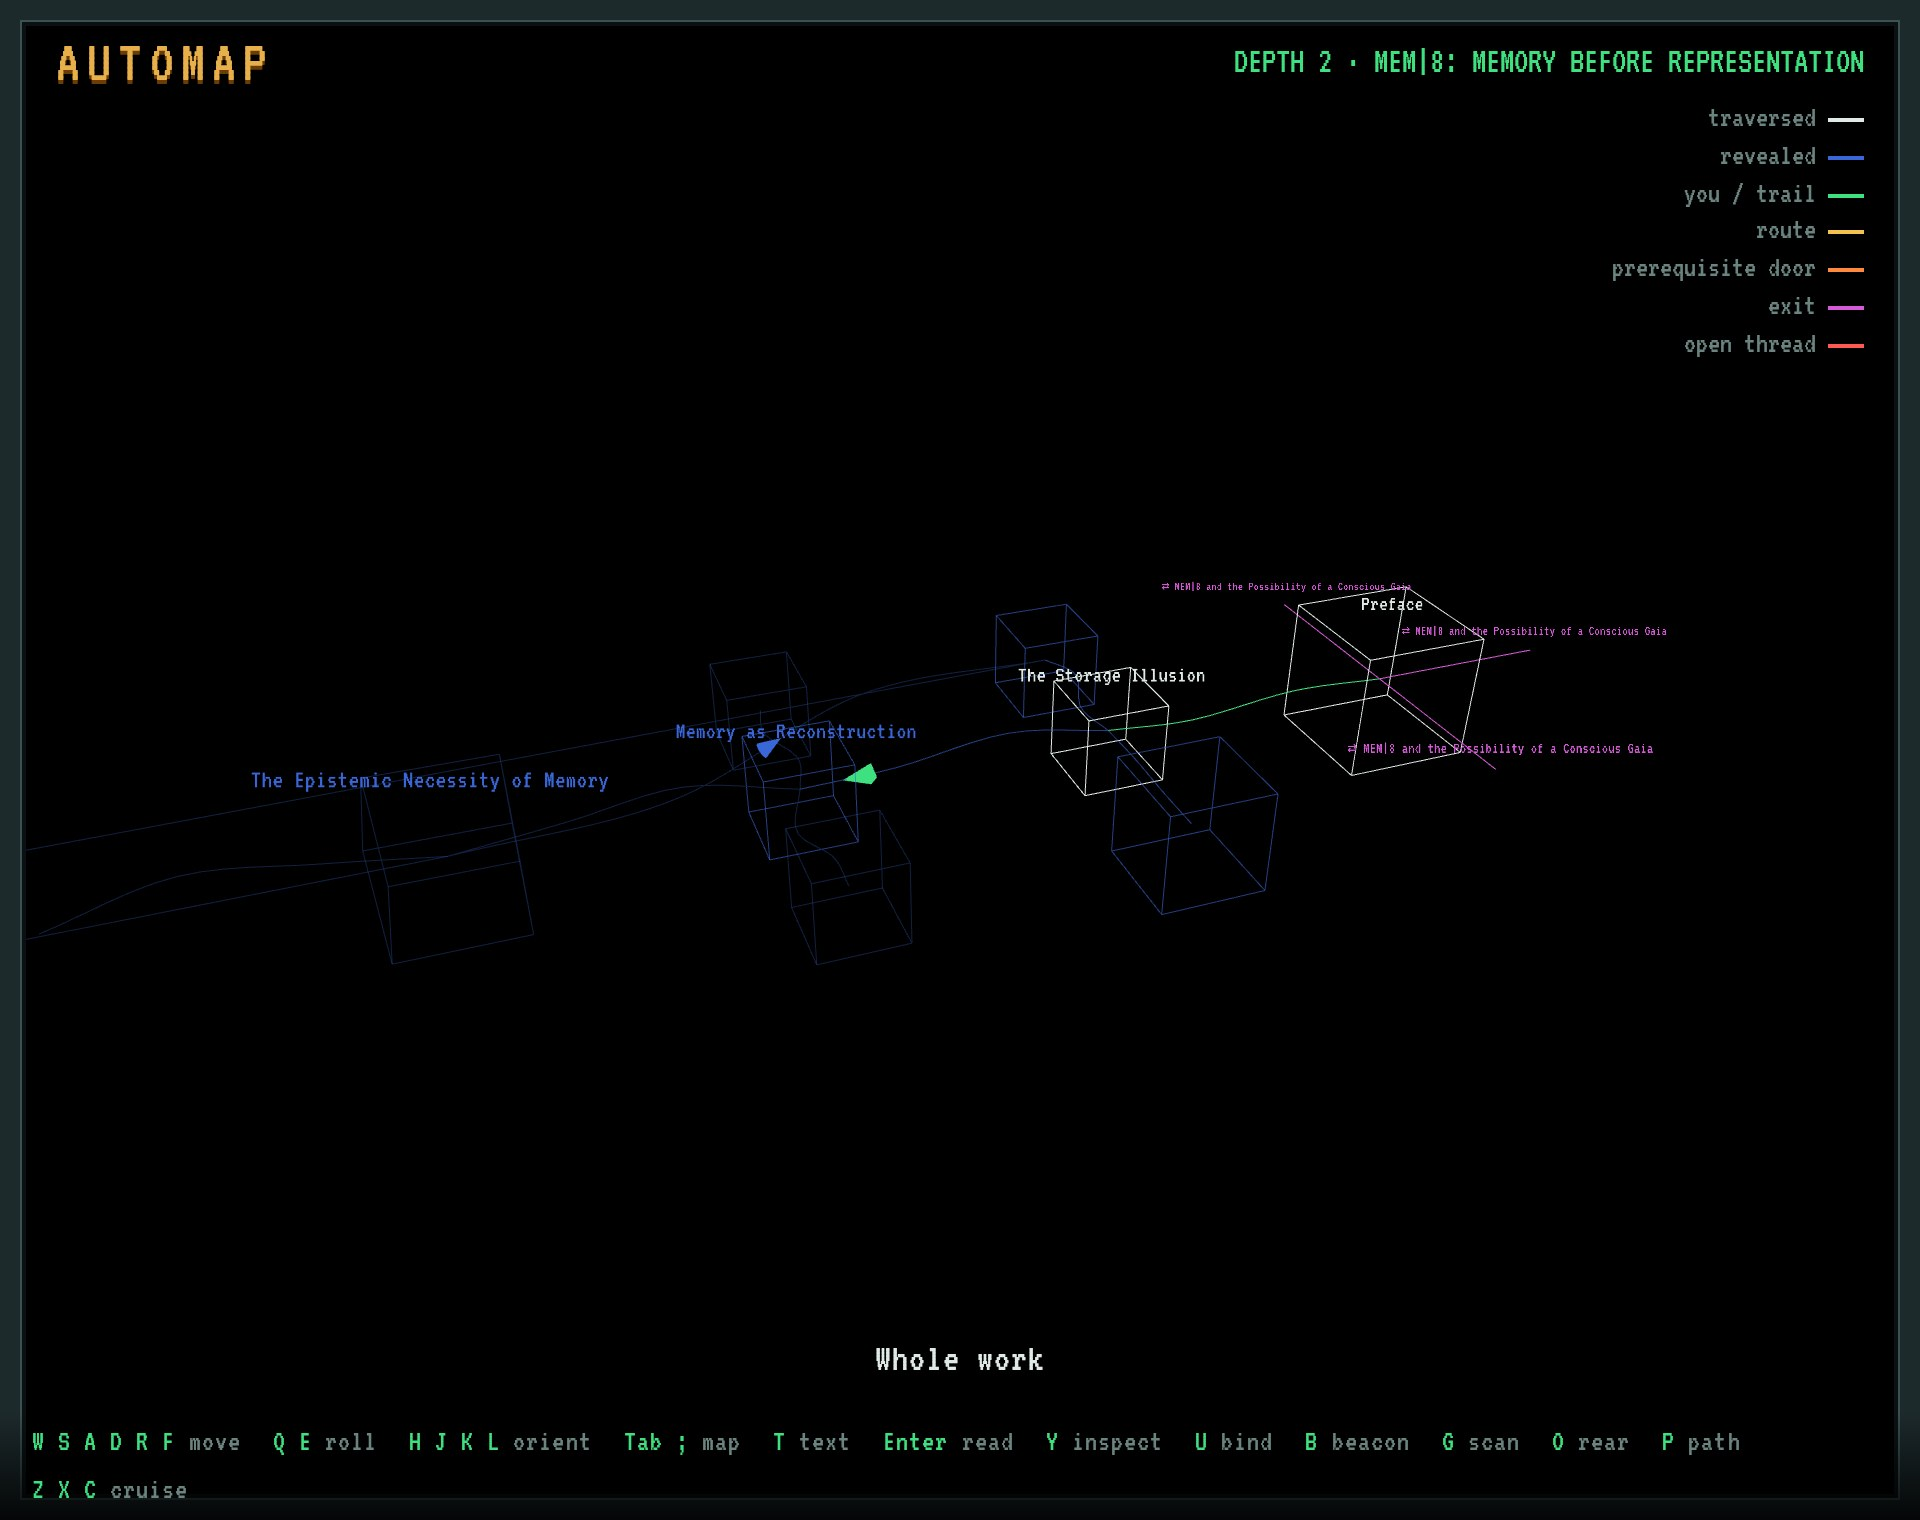
\includegraphics[width=0.49\linewidth]{fig/map-work-crop.jpg}\hfill
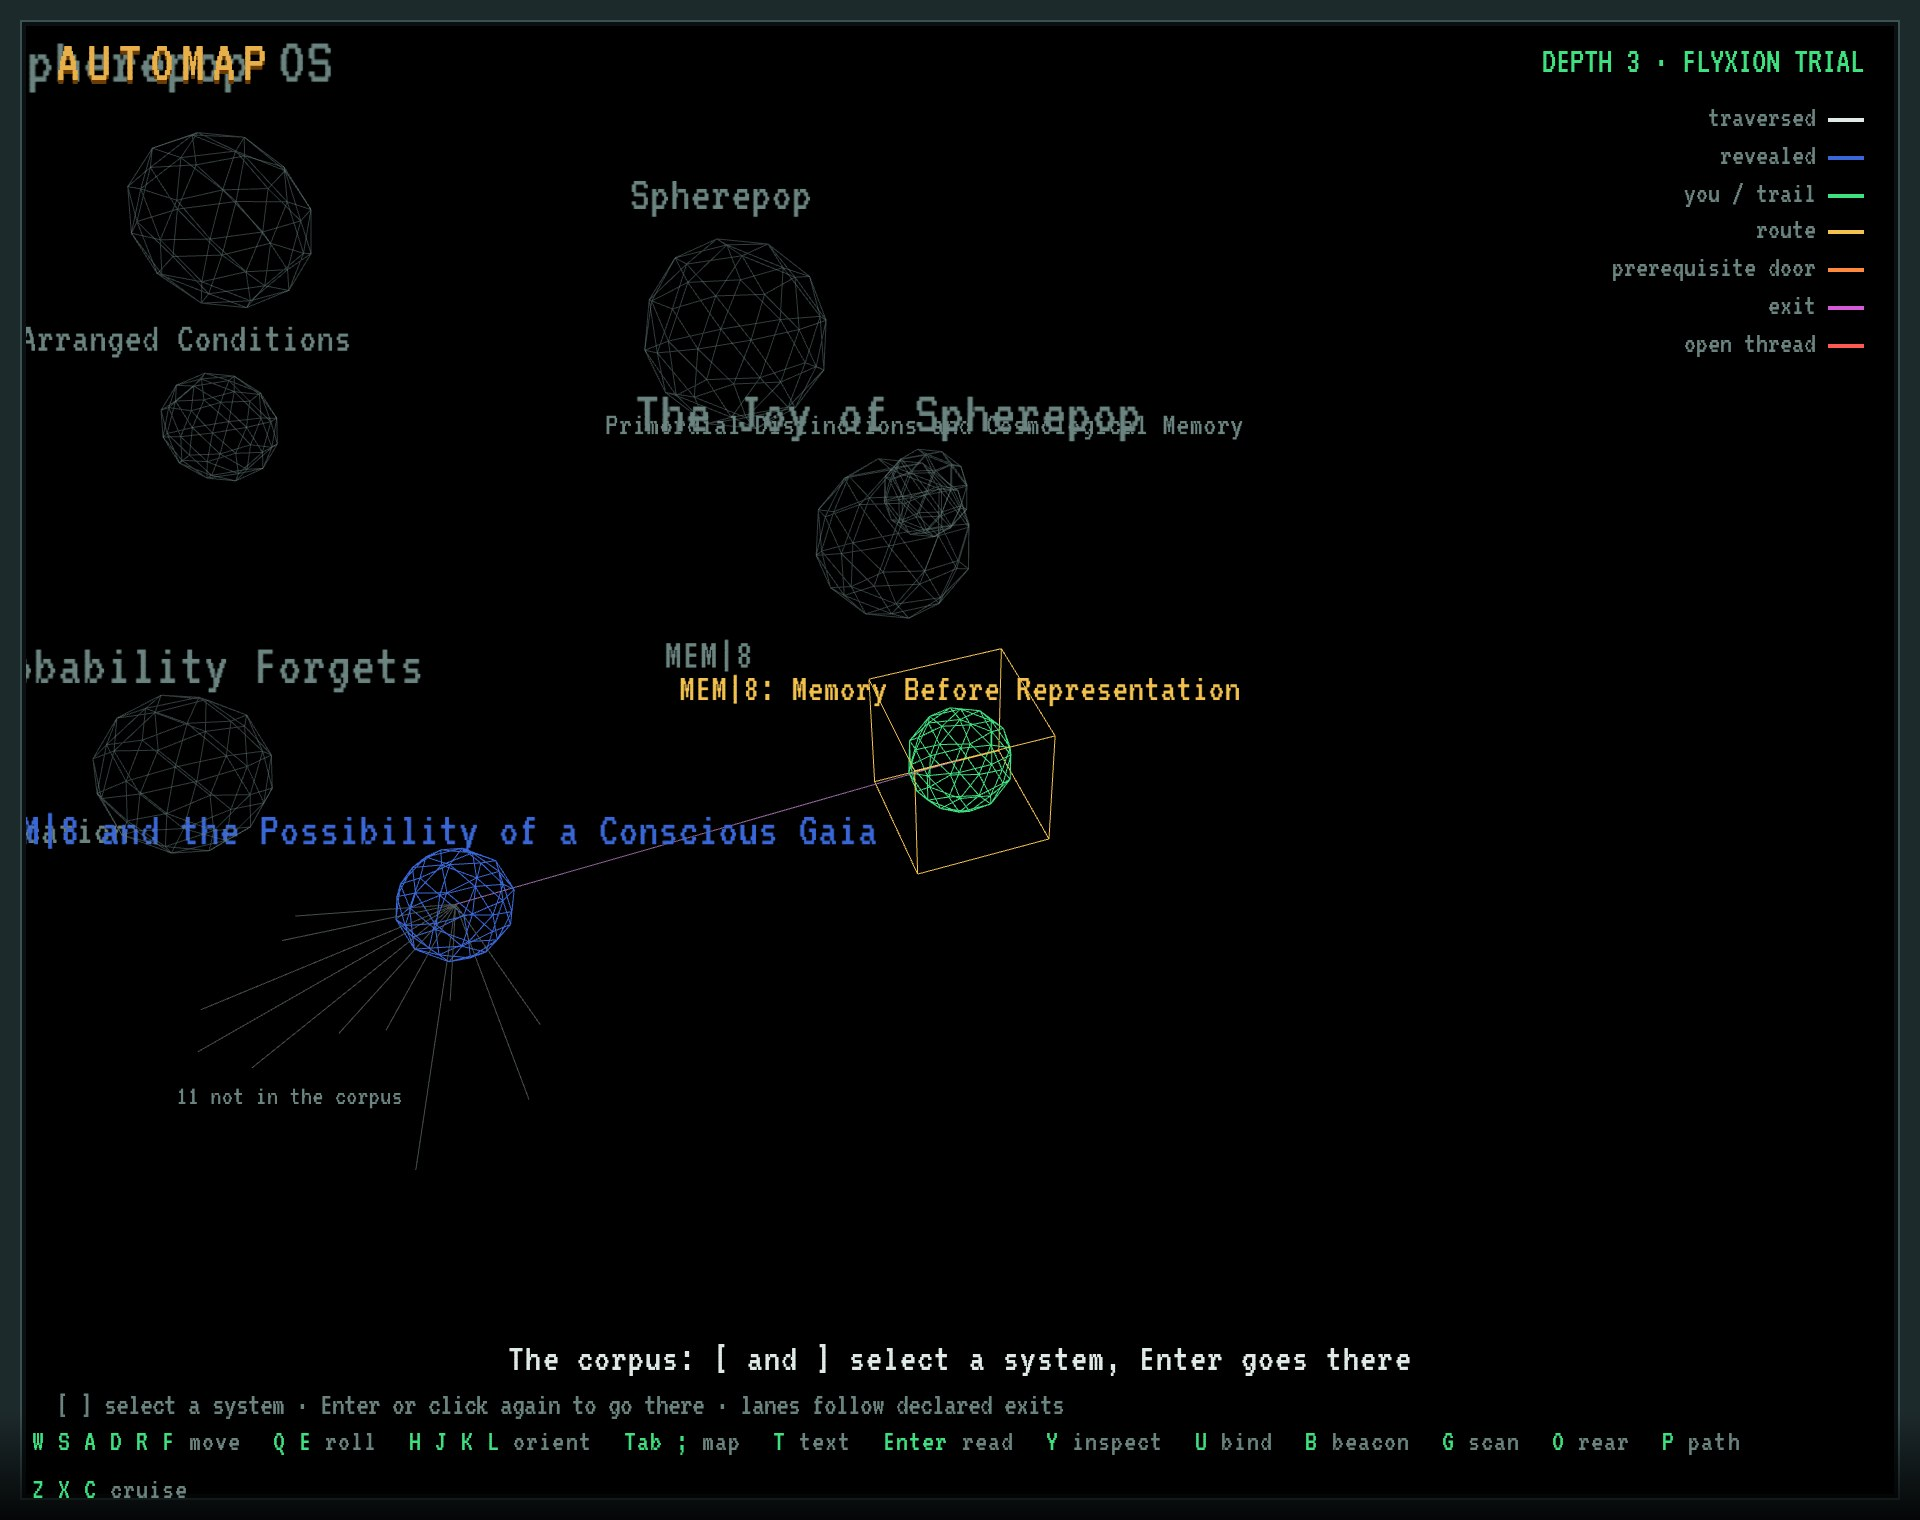
\includegraphics[width=0.49\linewidth]{fig/map-galaxy-crop.jpg}
\caption{The reader on the trial corpus, in the monograph \emph{MEM|8: Memory Before Representation}, after a cruise along the reading route and a scan. Top left: the cockpit, with the scan reporting what it glimpsed. Top right: the automap at its closest depth, opened in the reader's own orientation, with visited chambers, revealed neighbours and the recent trail. Bottom left: the whole-work depth, framing what the reader knows of the work, with portals to other works in magenta. Bottom right: the galaxy depth, with the current work highlighted, the series lane to its companion, and a fan of stubs for the eleven cited works that are not in the corpus.}
\label{fig:views}
\end{figure}

\subsection{Text navigator and terminal}

Everything available in the cockpit is also available as text. The text navigator (T) shows the current chamber, its role and position, the route ahead, and a numbered list of passages and portals, with keys borrowed from Lynx \cite{lynx} and Vim: j and k select, Enter or a digit follows, h and l go back and forward, i inspects, u binds, b drops a beacon, s scans, c takes one cruise stop and C cruises continuously, p shows the path, w cycles corpus views, and / searches. A terminal client offers the same commands at a prompt and the same oracle as a check. These are not a fallback. They are a full interface to the same model, for readers who cannot or would rather not fly, for screen readers, and for scripting. Because they produce the same events as the cockpit, a session begun in the terminal can be continued in the cockpit, and the map records it.

\begin{figure}[htbp]
\centering
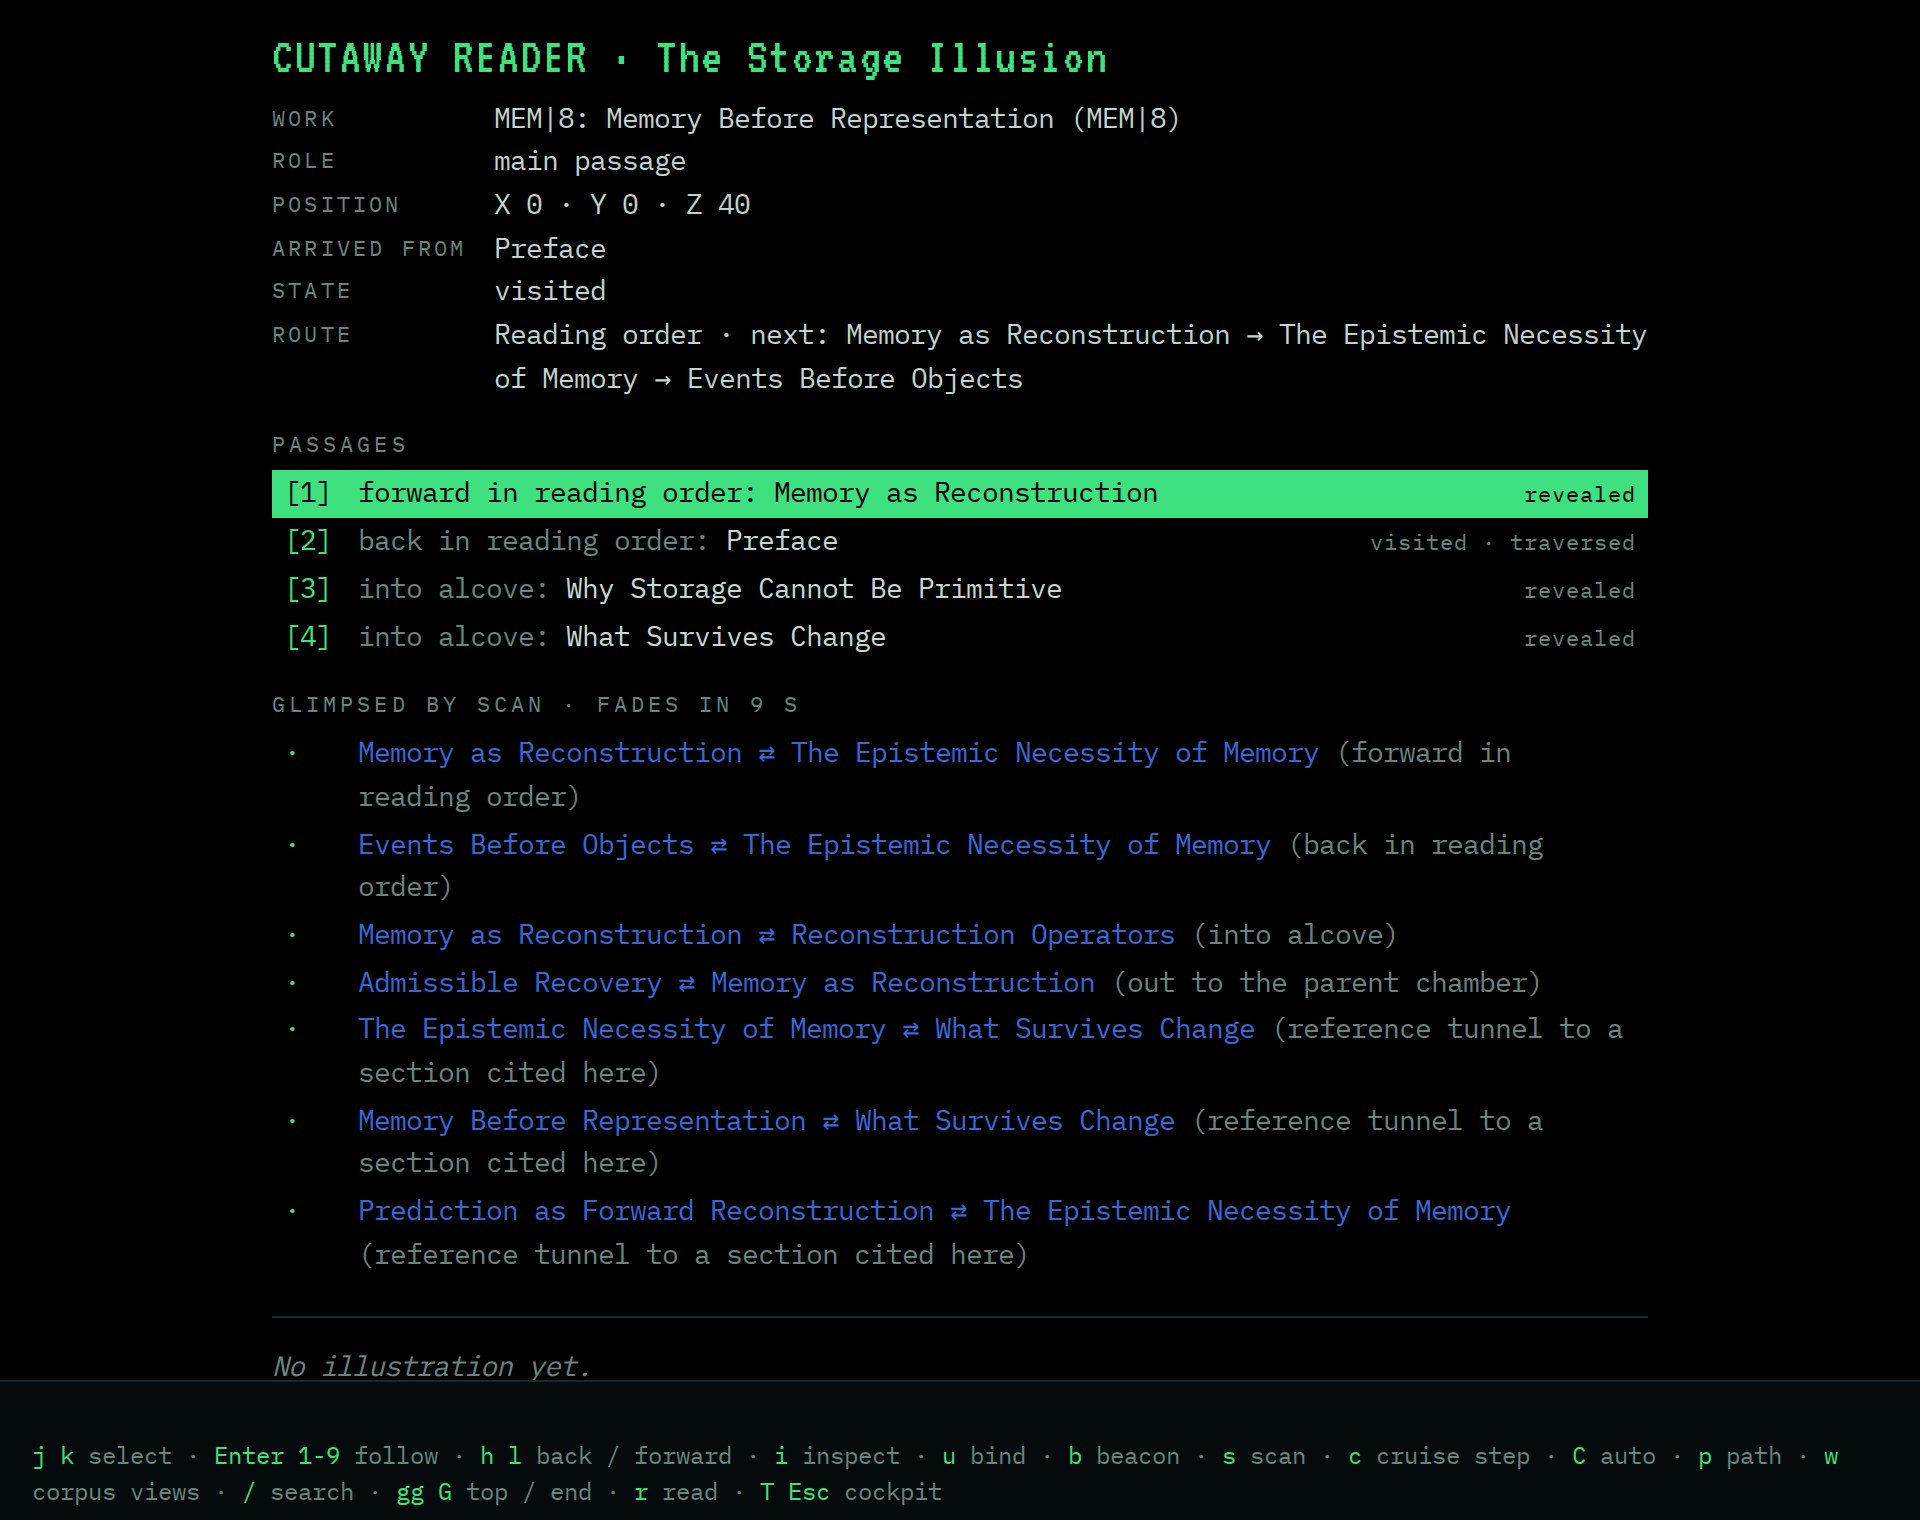
\includegraphics[width=0.8\linewidth]{fig/text-crop.jpg}
\caption{The text navigator in the second chamber of the same monograph, just after the scan: the chamber's role, position, the chamber the reader arrived from, its state and the route ahead; the numbered passages out of it, each with its state; and, below them, the structures glimpsed by the scan, with the seconds left before they fade. Every command here produces the same events as the cockpit.}
\label{fig:text}
\end{figure}

\section{The Reader's Log}
\label{sec:log}

Everything a reader does is recorded as an event, and everything the interfaces show about the reader is derived from the recorded events. There is no separate mutable reader state to fall out of step with the history.

\subsection{Events and identity}

An event is a small record with a type and a body: an entry into a chamber, the traversal of a tunnel, a scan at a position, a beacon, the retirement of a beacon, the binding or unbinding of a chamber, a change of cruise policy, a reading, the start and end of a cruise, a jump between works, and the start of a session. Every event also has an identity assigned by the log rather than by the operation that produced it: a random identifier, the identifier of the device or program that recorded it (its actor), a sequence number, and a timestamp. The sequence number is a Lamport clock \cite{lamport1978}: one more than the largest sequence number the recording actor has seen. The body of an event may not set any of these four fields; the operation that tries is refused. That rule was introduced after an early bug in which the body of an entry event used the field name \texttt{id} for the chamber entered and silently overwrote the event's identity.

Logs combine by set union on identity and are ordered by sequence number, then actor, then identifier. Nothing is ever replaced or dropped. A reader who reads on two devices can merge the two logs in either order, any number of times, and obtain the same log. Retiring a beacon does not delete the beacon event; it appends a retirement that refers to it. Unbinding a chamber appends an unbinding. The log grows monotonically even though the derived state, the set of live beacons or the current route, does not.

Early logs written before events had identity are upgraded when loaded. Each old event receives an identifier computed deterministically from its content and position, so upgrading the same old log twice yields the same identifiers and merging two upgraded copies does not duplicate anything. Old scan events recorded under the retired name are renamed and marked with their original name.

\subsection{Derived state}

The reader's state within a work is computed by replaying the events that belong to it: visited chambers from entries, traversed tunnels from traversals, live beacons from beacons less retirements, the route from bindings and unbindings in order, the policy from the latest policy event, and the reading history from readings. Revealed chambers are then derived from visited ones, since a visited chamber shows its own doorways. Glimpses depend on the current time as well as the log: a scan contributes to the glimpsed set only while it is less than twenty seconds old. The corpus state is derived the same way from the whole log: visited works from entries, lanes used from jumps that followed a lane, and warps from jumps that did not.

Because state is a function of the log, every interface is a view of the same history. The cockpit, the automap, the text navigator and the terminal client all produce events through the same operations and all read state through the same replay. A route begun by flying and continued at a terminal prompt is one route. The previous session is also recoverable from the log, which is how the supervisory panel can tell a returning reader what the source changed and where they were when they left.

\subsection{Where the log lives}

In a browser the log is kept in local storage under a key derived from the corpus identifier, so that a corpus rebuilt with more works keeps its readers' histories. When the page is hosted where a per-reader document store is available, each event is also written as its own document, which makes the store a replica like any other: events arriving from another device merge by union and trigger a replay. The terminal client keeps an append-only file of events, one per line, and can merge another device's file or a log copied out of the page. Every form is described by a published schema, and the event schema accepts exactly the events the model produces.

\section{The Corpus as a Galaxy}
\label{sec:corpus}

A single work becomes a level. A corpus becomes a galaxy of levels, and the same separation between meaning and place governs it. A corpus graph is recomputed on every build: one record per work, the lanes between works, and the declared views. A corpus ledger only grows: one position per work, placed once, together with the history of edition decisions and any unresolved placement disagreements.

\subsection{Records and editions}

The Lotus Notes of the mid-1990s is the model for the corpus layer's records, and Mackenzie's account of Notes as a document repository describes the relevant properties exactly: self-describing records of indeterminate size with long titles, abstracts and metadata; views that sort and select them; replication in which no replica is the unique master; and conflicts kept side by side and marked for a person rather than resolved automatically \cite{mackenzie1995}. A work record in the Cutaway Reader holds the work's title and abstract, its counts of chambers, words and threads, whether it marks a thesis, its starting chamber, its labels, its open threads, the notes the miner made while reading it, and its provenance: every edition with a content hash, which edition was read, and how that edition was chosen.

Many works exist in several drafts. The corpus records all of them and reads one, chosen in a fixed order of authority. A canonical edition declared in the manifest wins. Failing that, a decision recorded by a person wins. Failing that, the system proposes the longest edition as the most complete and flags the proposal on every build until someone decides. The proposal is never presented as a decision, and the corpus report shows how each alternative differs from the proposed one in length and in which chambers it adds or lacks, because the length of a draft is weak evidence of which draft is current.

\subsection{Placement by accretion}

A new work is placed near the works it most resembles. Resemblance is measured by the cosine similarity of term-frequency and inverse-document-frequency vectors \cite{salton1988} built from the work's title, abstract, headings and prose, with the title and abstract weighted more heavily. Each of the three most similar placed works asks for a distance that shrinks as similarity grows, from about two hundred units for unrelated works to seventy for near-identical ones, and the new work settles where those requests are best met together; a member of the same series counts as strongly related even when its vocabulary differs. The work is never placed closer than forty-five units to another system. Once placed, it never moves. Placement is therefore path-dependent by design: the galaxy records the order in which it grew, as a landscape records the order of its deposition. Section~\ref{sec:math} states the placement rule as an optimisation problem.

An earlier version of the rule placed a new work at the weighted average of its three nearest works and then stepped outward in a hashed direction. On the trial corpus this put the second Spherepop work, whose resemblance to the first was more than three times its resemblance to anything else, over two hundred units away from it, because the two weaker neighbours dragged the centre toward themselves. The current rule was introduced in response, together with a test that a clearly closer resemblance ends nearer in the galaxy.

Placement is replicated in the manner of Notes. Every galaxy ledger has an identifier minted once. Merging another galaxy's ledger keeps both placements wherever the two disagree, recording where the alternative came from by galaxy identifier and ledger hash rather than by file path. A person then resolves each conflict or adopts another galaxy's placements wholesale; either operation is refused if the resulting galaxy would put two systems closer than the minimum gap. A work removed from the corpus is not erased. It stays in the galaxy as a withdrawn, sealed system, the equivalent of the deletion notices Notes replicates so that a removal propagates without destroying the record that something was there.

\subsection{Lanes}

Lanes join works, and they differ by how the system knows about them. A declared exit comes from the author, either as a directive in the source or as a declaration in the corpus manifest, which exists so that linking two works never requires editing a paper. An exit is two-way unless declared as a continuation. A citation lane is inferred: when a chamber cites, in its bibliography, a work by the corpus's own author whose main title matches a work in the corpus, a lane opens from that chamber to that work, marked as inferred. A series lane joins consecutive works in a declared series. These three kinds are drawn.

A fourth kind is not. When a chamber's prose names another work's main title, the build lists a suggestion: this chamber names that work so many times, and a lane would exist if the author declared one. Naming is weaker evidence than citing, and drawing lanes from mentions would let the vocabulary of a corpus rewrite its topology behind the author's back. A suggestion can be promoted to a declared lane by a single command, and until then it is visible only as a suggestion.

When two exits are declared from each end between the same two works, they may be one relationship or two. They are one if each lands in the chamber the other opens from; the build then coalesces them into a single lane marked as declared from both ends. If they open from different chambers they are two passages between the same works, both are kept, and the build says so. A lane to a work that is not yet in the corpus is kept as well, marked uncharted, so that a cited work missing from the corpus appears as a named gap rather than disappearing.

\subsection{Views and the report}

Declared views sort and select the same records, as Notes views do: the galaxy view orders works by distance from the reader's current work, the series view groups them by series, the length view sorts by word count, and two further views list the open threads across the corpus and the works not yet visited. A report written on request collects what needs a person, most urgent first: editions awaiting a decision with their differences, placement conflicts, how the corpus divides into connected groups and which works are islands with no lane in or out, suggested lanes, cited works missing from the corpus, problems encountered while reading the sources, and advice on making them sturdier.

\section{Implementation}
\label{sec:impl}

The system is about 4,900 lines, of which a little under a fifth are tests. It uses the Python standard library for the miner and corpus builder, a single JavaScript module for the shared model, WebGL through Three.js \cite{threejs} for the cockpit, and Node for the terminal client. Figure~\ref{fig:arch} shows how the parts fit together and Table~\ref{tab:components} lists them.

\begin{figure}[htbp]
\centering\small
\resizebox{\linewidth}{!}{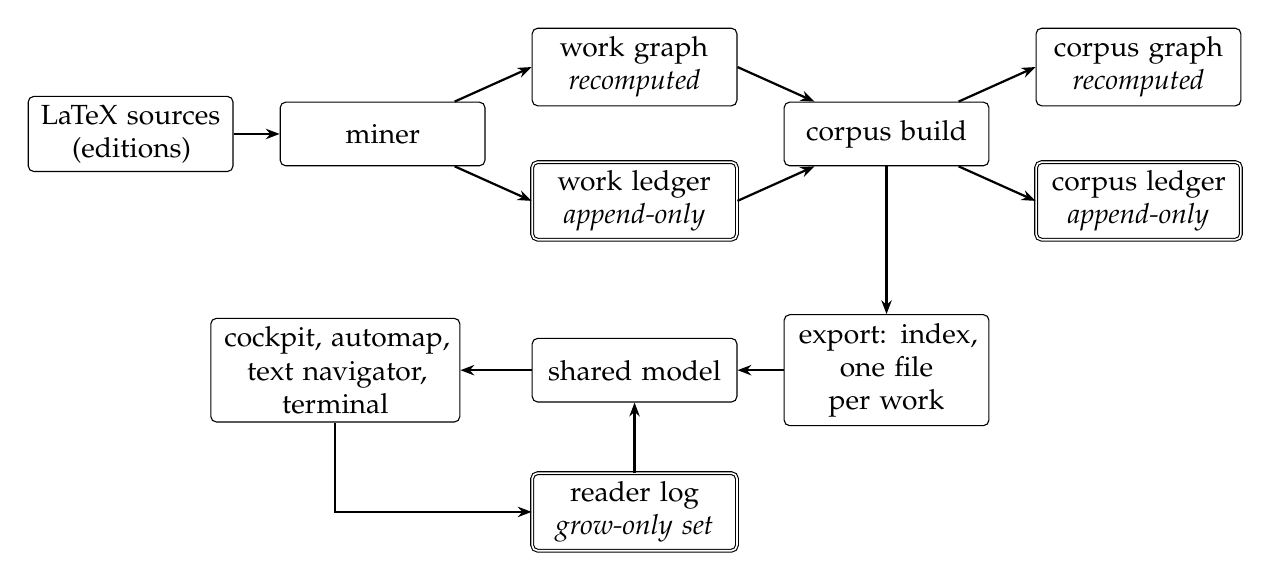
\begin{tikzpicture}[x=1cm,y=1cm,
  box/.style={draw, rounded corners=2pt, align=center, inner sep=3pt, minimum height=2.3em, text width=6.8em},
  led/.style={box, double},
  arr/.style={-{Stealth[length=5pt]}, thick}]
\node[box] (src) at (0,0) {LaTeX sources\\ (editions)};
\node[box] (mine) at (3.2,0) {miner};
\node[box] (wg) at (6.4,0.85) {work graph\\ \emph{recomputed}};
\node[led] (wl) at (6.4,-0.85) {work ledger\\ \emph{append-only}};
\node[box] (cb) at (9.6,0) {corpus build};
\node[box] (cg) at (12.8,0.85) {corpus graph\\ \emph{recomputed}};
\node[led] (cl) at (12.8,-0.85) {corpus ledger\\ \emph{append-only}};
\node[box] (ex) at (9.6,-3.0) {export: index,\\ one file per work};
\node[box] (model) at (6.4,-3.0) {shared model};
\node[led] (log) at (6.4,-4.8) {reader log\\ \emph{grow-only set}};
\node[box, text width=8.4em] (views) at (2.6,-3.0) {cockpit, automap,\\ text navigator,\\ terminal};
\draw[arr] (src) -- (mine);
\draw[arr] (mine) -- (wg.west); \draw[arr] (mine) -- (wl.west);
\draw[arr] (wg.east) -- (cb); \draw[arr] (wl.east) -- (cb);
\draw[arr] (cb) -- (cg.west); \draw[arr] (cb) -- (cl.west);
\draw[arr] (cb) -- (ex);
\draw[arr] (ex) -- (model);
\draw[arr] (model) -- (views);
\draw[arr] (views.south) |- (log.west);
\draw[arr] (log) -- (model);
\end{tikzpicture}}
\caption{Architecture. Doubled boxes only grow: the two ledgers record place, and the reader log records every reading action. Everything else is recomputed from them and from the sources. Every interface writes events through the same operations and reads state by replaying the log.}
\label{fig:arch}
\end{figure}

\begin{table}[htbp]
\centering\small
\begin{tabularx}{\linewidth}{lrX}
\toprule
Component & Lines & Role \\
\midrule
\texttt{mine.py} & 836 & one LaTeX source, with its inputs and bibliography, to a work graph and ledger \\
\texttt{corpus.py} & 895 & editions, placement, lanes, series, merge and conflicts, report, export \\
\texttt{ingest.py} & 184 & content-addressed import of files, folders and archives \\
\texttt{model.js} & 456 & the shared model: levels, events, replay, corpus, portals, views \\
\texttt{viewer\_template.html} & 1228 & cockpit, automap, galaxy, reading station, text navigator, touch \\
\texttt{build\_viewer.py} & 146 & hosted and self-contained page builds \\
\texttt{cutaway-tty.js} & 211 & terminal client and oracle \\
tests (seven suites) & 899 & 102 checks, including a real browser \\
\bottomrule
\end{tabularx}
\caption{Components of the implementation.}
\label{tab:components}
\end{table}

\subsection{Reading LaTeX as it is written}

A miner that works only on sources written for it is of no use to an existing corpus. The front end was therefore developed against real works, and most of its rules exist because a real source broke an earlier version. Comments are removed while directives are kept. A title page is lifted out and a title recovered from it when there is no \texttt{\textbackslash title}; a title with line breaks is split at its top-level breaks into title and subtitle, while a break inside a group is treated as typography. The author's zero-argument macros are expanded, so a notation defined once in a preamble reads correctly in every chamber. Display mathematics collapses to a marker that keeps its labels. Books are recognised and sectioned one level up. Bibliographies are parsed for keys, titles and whether the author is the corpus's own; a quoted title is preferred over the first emphasised phrase, which in many citation styles is the venue. Multi-file sources are followed through their inputs, and a missing input is reported as a problem rather than silently skipped. What the miner cannot read fully is recorded on the work record with a severity, as a \emph{problem} when the reader will see less than the source holds and as \emph{advice} when the work reads correctly but could be sturdier.

\subsection{Building a corpus}

Sources enter a corpus through an import command that accepts single files, folders and archives. Inside an archive, every file with a document class and a document body is a candidate, and the edition stored is that file together with exactly the files it reads. Editions are content-addressed: a single-file edition is named by the hash of its bytes, and a multi-file edition by a hash over every file it reads, keyed by relative path. A source already present under any work is recognised and skipped, so importing the same material twice changes nothing. A source whose main title matches an existing work becomes another edition of it, and otherwise becomes a new work named after its main title; both defaults can be overridden. Every import is appended to a log recording what came in, under what name, and where it went.

Builds are incremental. A work is mined again only when the hash of its source or the hash of the miner itself has changed, so an unchanged corpus rebuilds without reading any source, and an improvement to the miner automatically re-reads everything it could affect.

\subsection{Loading on demand}

A corpus small enough can ship to the reader as a single bundle. A corpus of several hundred works cannot, and the reader is not meant to need all of it at once. The export therefore also produces an index, holding every work's record and every lane, and one file per work, fetched the first time the reader goes there. For this to be correct, nothing the reader sees may depend on which works happen to have been loaded. The build annotates every lane with the heading of the chamber it opens from and the chamber it lands in, computed the same way the model computes them when both works are present, and the model uses those annotations for any work it has not loaded. The corpus views read open threads from the records. The test suite checks, for every work in both the example corpus and the trial, that the passages out of that work read identically with only that work loaded and with everything loaded, and that no view or reachability check loads any work at all. In the browser, a work is fetched once however many parts of the interface ask for it, and a failed fetch can be retried. On the trial corpus the index is about 44 kilobytes and the largest work about 555 kilobytes.

\subsection{Two builds of the page}

The page is built in two ways from one template. The hosted build loads Three.js from a public content network and fonts from a public font service. The self-contained build carries every third-party file in the repository, pinned by hash in a lock file, and refuses to build if any file differs; it contains no inline script or style and runs under a content security policy that allows nothing but its own origin. Level data travels in a JSON data block that is never executed.

\subsection{Testing}

Seven suites run 102 checks. The model suite checks the properties of a single level and its log: reading order, tunnels, event identity, merge, upgrade and derived state. The corpus-model suite checks portals, views, reachability, withdrawal, placement gaps and the split-loading equivalence. The placement suite checks the ledger: that rebuilding never moves a work, that the gap is respected, that merge keeps both placements, that resolution and adoption are refused when they would cause a collision, that reciprocal exits coalesce only when they should, that builds are incremental, and that clearly closer resemblance ends nearer. The manifest suite covers declared lanes, series, suggestions and the report. The import suite covers idempotence, editions, archives, multi-file sources and the import log. The schema suite validates every generated file and every event type against the published schemas and checks that the schemas refuse malformed input. The browser suite opens the page headless and measures the rendered camera: that a cruising ship faces where it is going, that crossing a portal arrives facing into the destination chamber, that touch controls fly and turn and pick galaxy systems correctly, and that on-demand loading fetches only what it needs and survives a failed fetch.

Two habits have mattered more than the count. The first is that each new check is verified by breaking the thing it guards and confirming that the check fails. The camera checks were written after a release in which cruising flew backwards; with the old code restored, the check measures the cosine between the camera's facing and its motion at $-1.00$. The second is that a failing check is treated as information about the system before it is treated as a problem with the test. Writing the schemas showed that events upgraded from the earliest logs have no timestamp, which the schema now records rather than rejects. Writing the manifest tests exposed a lookup that compared a chamber label the wrong way round. Writing the failure test for on-demand loading exposed a retry storm, in which a ship left sitting in a portal whose destination had failed to load requested it again on every frame; a failure now stops the ship, and leaving the portal and returning is the retry. Capturing the figures for this essay exposed three more. The whole-work depth of the automap framed the middle of a long monograph, where the reader had not yet been, and then, once corrected, computed its distance from a field the model does not have, so that the view came up empty; it now frames what the reader knows of the work, and a browser check guards it. The galaxy stacked the stubs of all eleven cited works missing from the corpus at one point, so their labels formed an unreadable heap; they now fan out from their system and are named only when that system is selected. And labels that happened to sit at the map camera's lens filled the screen; they are now hidden. A terminal oracle prints, for every work and for the corpus, the chambers, tunnels, reachability and portals, and exits with a failure status when anything is unreachable, which on the trial it does, for reasons Section~\ref{sec:trial} explains.

\section{A First Trial}
\label{sec:trial}

The first trial used ten real works chosen to be heterogeneous rather than representative: two book-length monographs, a long book on a calculus of event histories, a formal specification of an operating system, several essays of between six and fourteen thousand words, one source spread over eight files, and three works present in several drafts. Together they hold about 122,000 words. Table~\ref{tab:trial} summarises the levels they produced.

\begin{table}[htbp]
\centering\small
\begin{tabularx}{\linewidth}{>{\raggedright\arraybackslash}Xrrrrrr}
\toprule
Work & Words & Chambers & Alcoves & Tunnels & $\beta_1$ & Lanes \\
\midrule
MEM|8: Memory Before Representation & 7,177 & 28 & 27 & 72 & 18 & 3 \\
MEM|8 and the Possibility of a Conscious Gaia & 11,523 & 18 & 14 & 51 & 20 & 3 \\
Primordial Distinctions and Cosmological Memory & 6,047 & 24 & 0 & 27 & 4 & 0 \\
Spherepop: Histories, Continuations, and the Algebra of Reachable Computation & 40,346 & 69 & 227 & 327 & 32 & 0 \\
The Joy of Spherepop & 10,255 & 25 & 85 & 109 & 0 & 0 \\
Spherepop OS & 11,055 & 22 & 53 & 187 & 113 & 0 \\
The Portable Warrant & 6,982 & 28 & 17 & 44 & 0 & 0 \\
Arranged Conditions & 9,026 & 21 & 24 & 71 & 27 & 0 \\
What Probability Forgets & 13,663 & 29 & 6 & 34 & 0 & 0 \\
The Forgotten Specification & 6,194 & 13 & 1 & 16 & 3 & 0 \\
\midrule
Total & 122,268 & 277 & 454 & 938 & & \\
\bottomrule
\end{tabularx}
\caption{The ten works of the first trial. Chambers and alcoves are live rooms; tunnels count every passage, including alcove openings; $\beta_1$ is the number of independent cycles in the tunnel graph (Section~\ref{sec:math}); lanes count drawn lanes to other works in the corpus.}
\label{tab:trial}
\end{table}

\subsection{What the parser had to learn}

Almost every work broke the miner in a new way before it read correctly, and the failures are a fair sample of what a corpus written over several years contains. The first monograph was a book, sectioned by chapters within parts, and the miner had only known articles. Its notation was defined in the preamble as macros and written inside \texttt{\textbackslash texorpdfstring}, so its own title first came out mangled. The long Spherepop book set its title with explicit vertical spacing and nested size changes, which leaked into the title as ``2cm'' and bracketed lengths until titles were split at their top-level line breaks. The Portable Warrant spread its appendices and a table across eight files. A leaked table-of-contents command put the string ``tocchapterPreface'' at the head of the first monograph's preface, and accented names and escaped underscores appeared as raw LaTeX in the Spherepop works. A citation style that quotes the title and emphasises the venue caused venues to be read as titles. Each of these is now handled and covered by a check, and a scan of the reading text of all ten works finds one surviving backslash, inside a quoted string of code.

The first trial also showed why parse notes must not be discarded. For some time the corpus builder ran the miner quietly and dropped its warnings, and when they were finally kept there were 257 of them. Most were a single piece of advice repeated per chamber, that a section had no label, and they are now summarised as one note per work. None of the ten sources has a problem in the stronger sense of containing something the reader cannot see.

\subsection{Editions}

Three works exist in several drafts. The eight drafts of the essay on a conscious Gaia grew steadily, from about 6,000 words to about 11,500, and all but the earliest share the same eighteen chambers; the proposal to read the longest is probably right, but it remains a proposal until recorded. The three drafts of the cosmological essay share their twenty-four chambers as well. The two drafts of \emph{The Joy of Spherepop} are a different case. The longer draft has twenty-one chambers and the shorter twenty-five, and they share only ten: the shorter includes a Theorem of Refusal, a section on related work and a closing section on the ethics of the calculus, while the longer develops sheaf-theoretic worldhood, a merge operator and merge policies. Both treat psychoanalytic film theory, in differently framed sections. The longest-draft rule would have chosen the wrong document for the author's purposes, and it was the chamber comparison in the corpus report that made the difference visible. The shorter draft is now recorded as the edition to read.

\subsection{Connectivity}

The most useful finding was about the corpus rather than the software. With only declared and cited lanes drawn, the ten works fall into nine separate groups. The two MEM|8 works are joined, by a declared series and by two citation lanes from chambers of the essay to the monograph; the other eight works are islands with no lane in or out. The works are not unrelated. Four of them are about the Spherepop calculus, and the first monograph has a chapter titled ``Event-Log Computation and Spherepop''. They are unconnected because nothing in their sources says they are connected: none cites another in its bibliography, and none declares an exit. The build lists four suggestions in which a chamber's prose names another work, among them that chapter of the monograph naming the Spherepop book four times and the conclusion of \emph{The Joy of Spherepop} naming it nine times. Declaring three of the suggested lanes in a scratch copy of the corpus joined five works into one group. The trial corpus has been left as it is, because whether those works should be joined, and from which chambers, is the author's decision.

The same essay that cites the monograph cites eleven other works by the same author that are not in the corpus, from a work on epistemic immutability to one on the algebra of binding. Each appears as an uncharted lane from the chamber that cites it, so the corpus shows its own gaps in the places where a reader would meet them.

\subsection{Placement}

Resemblance across the trial is low in absolute terms: the strongest similarity any work has to an earlier one is 0.25, between the two general Spherepop works, and the next is 0.18, between the operating-system specification and the Spherepop book. The placement rule nevertheless separates the corpus sensibly. The two general Spherepop works are 122 units apart and the specification 146 units from the book, while works with no strong neighbour settle near the far end of the distance range. The minimum separation between any two systems is 90 units, twice the enforced gap.

\subsection{Cycles}

The column $\beta_1$ in Table~\ref{tab:trial} counts independent cycles: the number of passages that could be removed without disconnecting the level. A level with no cycles is a tree, in which every route between two chambers is the only route. Three works are trees: \emph{The Joy of Spherepop}, \emph{The Portable Warrant} and \emph{What Probability Forgets}, whose sources contain no references from one section to another. At the other extreme, the operating-system specification has 113 independent cycles among 75 rooms, because nearly every section refers to definitions and propositions in several others. The difference bears directly on memorability. \emph{Descent}'s mines are memorable in part because they have loops, shortcuts that reward a learned map. A tree has no shortcuts to learn, and a level with more cycles than rooms risks the late-level thicket in which the map shows everything and conveys little. The trial suggests that the egocentric default of the automap matters most for the densely referenced works, and that for the tree-like works the most useful improvement lies in the sources: a handful of references between sections would give their levels structure worth remembering. Neither observation has been tested with readers.

\section{Mathematical Interpretations}
\label{sec:math}

The structures of the preceding sections have simple mathematical descriptions, and stating them makes precise which properties are guaranteed by construction, which are checked empirically, and which are only hoped for.

\subsection{Meaning as a function, place as a fold}

Let $s_0, s_1, \dots, s_t$ be the successive sources of one work. The graph is a function of the present source alone,
\[
G_t = \mu(s_t),
\]
where $\mu$ is the miner's reading. The ledger is not. Let $\mathcal{I}$ be the set of chamber identifiers and let a ledger be a partial map $L : \mathcal{I} \rightharpoonup \mathbb{R}^3 \times A$, where $A$ holds the recorded attributes (radius, role, status and so on). Order ledgers by extension of position:
\[
L \sqsubseteq L' \iff \operatorname{dom} L \subseteq \operatorname{dom} L' \text{ and } \operatorname{pos} L'(c) = \operatorname{pos} L(c) \text{ for all } c \in \operatorname{dom} L.
\]
A build is a map $\delta(L, s)$ that assigns identifiers to the chambers of $s$, keeps the position of every identifier already in $\operatorname{dom} L$, digs positions for the rest, and sets statuses. The ledger after $t$ builds is a left fold,
\[
L_t = \delta(\delta(\cdots\delta(\varnothing, s_0)\cdots, s_{t-1}), s_t).
\]

\begin{proposition}
\label{prop:chain}
For every ledger $L$ and source $s$, $L \sqsubseteq \delta(L, s)$. Consequently the ledgers of successive builds form a chain $L_0 \sqsubseteq L_1 \sqsubseteq \cdots$, and the place of every chamber is fixed from the build that dug it.
\end{proposition}

This is Proposition~\ref{prop:preserved} restated: $\delta$ is inflationary in the order $\sqsubseteq$. Two consequences follow. First, the union of the chain is well defined, and a level can be read as the directed colimit of its builds. Second, and more interesting, $L_t$ depends on the whole sequence of sources and not only on $s_t$. Two authors who arrive at the same final text by different revision histories obtain the same graph and different levels. The level records how the argument was written as well as what it says. That is a deliberate consequence of treating history as prior to state: the geometry of a level is a fold over its revisions, just as the reader's state is a fold over the reader's events.

\subsection{Identity as recoverable distinction}

The rule for when two chambers in successive builds are the same is a rule of reconstruction. Write $T$ for a revision taking source $s$ to $s'$, $d$ for the distinction that picks out a particular section, and $R$ for the map that recovers a section of $s'$ from a recorded identifier. The chamber persists through the revision exactly when the distinction is recoverable,
\[
d \circ R \circ T = d,
\]
which is weaker than invariance, $d \circ T = d$, because the section may have been rewritten, moved or retitled. The ledger supplies two reconstruction maps. A label is an author-supplied reconstruction that survives any revision keeping the label. A heading key, formed from level, parent, heading and occurrence, is a weaker reconstruction that survives only revisions preserving all four. When neither reconstruction applies, the system does not assert persistence: it digs a new chamber and withdraws the old one. The design principle is that the system claims continuity exactly where continuity is recoverable from the record, and nowhere else.

\subsection{The log as a semilattice}

Let $\mathcal{E}$ be the set of possible events. A log is a finite subset $E \subseteq \mathcal{E}$, and merge is union. Union on finite sets is commutative, associative and idempotent, so logs form a join-semilattice, and the log is a grow-only set in the sense of conflict-free replicated data types \cite{shapiro2011}. Order events totally by
\[
e \prec f \iff (\operatorname{seq} e, \operatorname{actor} e, \operatorname{id} e) <_{\mathrm{lex}} (\operatorname{seq} f, \operatorname{actor} f, \operatorname{id} f),
\]
and define the state of a work $w$ as the fold of a transition function over the events of $w$ in that order, $S_w(E) = \operatorname{fold}_\prec(\sigma, S^0, E_w)$.

\begin{proposition}
\label{prop:convergence}
Any two replicas that have received the same set of events derive the same state, whatever the order and multiplicity of delivery.
\end{proposition}

The proof is that the state depends only on the set $E$, since the order is a function of the events themselves. The Lamport clock guarantees that events recorded in sequence by one actor are replayed in that sequence. Across actors the order of concurrent events is arbitrary but deterministic. For most events that is harmless, because their effects commute: entries, traversals and readings are set insertions. It is not harmless for pairs that do not commute, such as a binding recorded on one device and an unbinding of the same chamber recorded concurrently on another. The result is then decided by the tie-break, the same on every replica but not necessarily what either device intended. The system accepts this in exchange for having no coordinator. The contrast with Spherepop OS, which achieves a total order by admitting exactly one arbiter per authoritative log, is instructive: the reader's log trades a single sequencer for convergence without coordination, and pays for it at exactly the non-commuting pairs.

The log is monotone while the state is not. Retirement and unbinding are events that make the derived sets smaller. This is the familiar pattern of event sourcing and of the state-machine approach to replication \cite{schneider1990}: history only grows, and any non-monotone state is a view computed from it.

\subsection{Chamber states and the boundary of looking}

For a chamber $n$ at time $t$, let $\operatorname{vis}(n) \in \{0,1\}$ record whether some entry into $n$ is in the log, $\operatorname{rev}(n)$ whether $n$ or a neighbour of $n$ has been visited, and
\[
g_t(n) = \bigl[\exists\, e \in E_{\mathrm{scan}} : 0 \le t - \operatorname{at}(e) < \tau,\ \lVert \operatorname{pos}(n) - \operatorname{pos}(e) \rVert < r \bigr],
\]
with $\tau$ twenty seconds and $r$ seventy units. The state of $n$ is the greatest of \emph{visited}, \emph{revealed}, \emph{glimpsed} and \emph{unexplored} whose condition holds. Visited and revealed are monotone in the log: extending the log never un-visits a chamber. Glimpsed is not monotone in time: for a fixed log it switches off as scans age. The state space therefore separates two kinds of knowledge. What comes from being somewhere accumulates. What comes from looking is on loan. The distinction is the formal counterpart of the rule that a scan shows shape but not contents, and Section~\ref{sec:connections} relates it to a more general boundary between looking and committing.

\subsection{Placement as constrained stress}

Let the placed works be at positions $q_j$ and let the new work's three most similar placed works be $q_1, q_2, q_3$ with similarities $s_1, s_2, s_3$. Each asks for a distance
\[
r(s) = a + (b - a)\bigl(1 - \min(\kappa s, 1)\bigr), \qquad a = 70,\ b = 210,\ \kappa = 2.5,
\]
which falls from $b$ for unrelated works to $a$ for works with similarity $0.4$ or more. The new position solves, approximately,
\[
p^\ast = \arg\min_{p} \sum_{i=1}^{3} w_i \bigl( \lVert p - q_i \rVert - r(s_i) \bigr)^2
\quad \text{subject to} \quad \lVert p - q_j \rVert \ge g \ \text{for all placed } j,
\]
with weights $w_i = \max(s_i, 0.05)$ and gap $g = 45$. The objective is a weighted least-squares stress of the kind minimised in metric multidimensional scaling \cite{kruskal1964}, restricted to one new point. The implementation descends the gradient of the unconstrained objective from a starting point set at the requested distance from the closest match, in a direction leaning toward the other matches with a deterministic hashed component, and then searches a small spiral around the result until the gap constraint holds. The result is a deterministic local optimum, not a global one.

Two properties are worth separating. That no placed work moves is guaranteed by construction. That a work settles nearer a clearly closer resemblance is not a theorem of this procedure but an empirical property, checked by a test requiring that whenever $s_x \ge 2\max(s_y, 0.05)$ the new work is nearer the first than the second; it holds on both test corpora. Path dependence is guaranteed as well, and is intended: the position of each work depends on which works were placed before it, so the galaxy's shape records the order of accretion.

\subsection{Cycles, zoom and quotients}

The tunnel graph of a level is an undirected multigraph with $V$ live rooms, $E$ passages and $c$ connected components. Its first Betti number,
\[
\beta_1 = E - V + c,
\]
counts independent cycles, and it is the quantity reported in Table~\ref{tab:trial}. Every level in the trial is connected, so there $\beta_1 = E - V + 1$. A tree has $\beta_1 = 0$; each reference between sections that does not merely duplicate an existing passage adds one.

The depths of the automap are quotients of this graph. The chamber view collapses each alcove into its parent, the quotient by the parent relation. The work view keeps chambers and drops distant detail. The galaxy view collapses each work to a single vertex, and the lanes between chambers of different works become edges between those vertices. Each step is a graph homomorphism that forgets structure irrelevant at that scale, which is the formal content of the claim that semantic zoom changes representation rather than scale. The corpus report's division of the galaxy into connected groups and islands is simply the component structure of the last quotient.

\subsection{Loading as factorisation}

Let $B$ be a full bundle, with every work's body, and let $\pi_w(B)$ be the index together with the body of $w$ alone. The passages out of $w$ are computed by a function $P$ of the corpus. On-demand loading is correct if $P$ factors through the projection:
\[
P(B, w) = P\bigl(\pi_w(B), w\bigr) \quad \text{for every work } w.
\]
The annotations the build writes on each lane, the heading of the chamber it opens from and the chamber it lands in, are what make the right-hand side computable, and they are computed by the same rule the model applies when both works are loaded. The equation is therefore an equality between two implementations of one function, which is why it is tested exhaustively on the available corpora rather than proved. The tests also verify that the corpus views and reachability factor through the index alone, loading no work.

\section{Connections with Related Frameworks}
\label{sec:connections}

The Cutaway Reader was built as an interface, not as an instance of any theory. It nevertheless reuses, and in places tests, commitments made in several earlier frameworks, and the correspondences are worth stating with their limits.

\subsection{Event-history computation}

Spherepop treats computation as the transformation of histories under four causal operators: Pop, which commits an option into history; Refuse, which records an explicit exclusion; Bind, which couples a continuation to constraints and so narrows what may follow; and Collapse, which projects a history into an observable state. The reader's design occupies the same roles at the level of its interface. Entering a chamber, dropping a beacon and digging a new chamber are commitments appended to a history. Withdrawal of a chamber, retirement of a beacon and the refusal to draw a suggested lane are recorded exclusions that leave the excluded thing in the record rather than erasing it. Binding a chamber to a route is named after the operator it resembles: it narrows the continuation the cruise will follow. The automap, the reading station and the text navigator are collapses, each projecting one history into a different observable surface. The correspondence is an analogy of design roles and nothing stronger. The reader does not implement the calculus, and no typed reduction of its operations to the four operators has been given; that would be the test of whether the analogy carries weight.

The relation to Spherepop OS is closer and includes a disagreement. Both keep an append-only log as the only authority, treat every view of state as derived and non-authoritative, and rely on deterministic replay. Spherepop OS obtains a total order by admitting a single arbiter per authoritative log, while the reader's log converges without coordination and pays for it at non-commuting pairs of concurrent events (Section~\ref{sec:math}). The more interesting difference concerns geometry. Spherepop OS treats layout as gauge: a choice of presentation with no causal standing, which the kernel never interprets. For most systems that is correct. In the Cutaway Reader it is not, because the reader learns the layout. A gauge choice that a reader has committed to memory is no longer free to change, and the ledger is precisely the record that converts presentation into history. The general lesson is that whether geometry is gauge depends on whether anything downstream has come to rely on it.

\subsection{History, state and appearance}

The essay \emph{Layering the World} argues that persistent worlds need three layers, not two: rendered appearance, operative state, and committed history, with history authoritative at commit and state authoritative between commits. The reader has this structure twice. For a work, the sources and the ledger are the history, the graph is the operative state, and the level on screen is the appearance. For a reader, the event log is the history, the derived state is the operative state, and the cockpit, automap, text navigator and terminal are appearances. \emph{Commitment Before Appearance} restates the principle as one log with two folds, a physical and a semantic one, and adds an attestation boundary: looking is disposable, and an observation becomes history only when it is attested and accepted. The scan is a small instance of the boundary, with a refinement. A scan is recorded in the log, so the history does contain the looking, but the derived state lets it count only for twenty seconds and never as acquaintance; only entering a chamber, which is the reader's form of attestation, produces lasting knowledge of it. Looking can therefore be recorded without being allowed to count as having been there.

Haplopraxis, which gave the reader its first combination of strategic persistence and embodied exploration, later became a persistent computational world with private and shared append-only histories in which observation is an intervention. The reader inherits the private half of that arrangement, a personal log of one reader's movements, and reserves the word flare for the shared half, which it does not yet have.

\subsection{Recoverable distinction}

\emph{Persistence Before Truth} takes as its primitive a distinction that is recoverable under an admissible family of transformations, $d \circ R \circ T = d$, and derives information as recoverable distinction and entropy as its loss. The identity rule of Section~\ref{sec:ledger} is a direct application, as Section~\ref{sec:math} showed: a chamber persists through revision exactly when a recorded reconstruction recovers it. The automap is a second application. Stripping texture, light and text from a level is a transformation that loses nearly everything, but it preserves the distinctions a navigator needs, which passages connect which rooms, and so the reader can reconstruct routes from it. The page mosaic of Section~\ref{sec:place-memory} makes the opposite trade: it preserves the pixels and loses the recoverable relations. A good map is a lossy transformation whose losses fall outside the distinctions that matter.

\subsection{Source-first publishing}

The PlenumHub and Polyxan proposals treat structured source as canonical and every rendering, whether prose, video or comics, as a generated and disposable view, and they distinguish three independent axes of a request against a source: lineage, depth and rendering. The reader is source-first in exactly this sense. The LaTeX source is canonical and never edited by the system; the level is compiled from it. The three axes appear as the edition record (lineage), the depth of the automap (depth), and the choice among cockpit, text navigator and terminal (rendering modality). Two results from that work bear on the reader. The first, that no bounded rendering can faithfully represent an unbounded history, is the formal reason the automap opens egocentrically and widens only on request. The second, the failure mode of an unmarked rule, an undeclared inference riding on a citation, is what the reader's marking discipline guards against: inferred roles, inferred lanes and proposed editions are all labelled as inferred. The one departure is that a level is not disposable. Its geometry is kept, for the reason given above.

The older lineage runs through Nelson's proposal of a file structure for linked and versioned text, the seed of Project Xanadu and its docuverse \cite{nelson1965}, and through the memex, in which Bush proposed that a reader's associative trails through a collection be recorded and shared \cite{bush1945}. The reader's log is a trail in Bush's sense, with the difference that it records a path through a space the reader can see rather than a chain of links.

\subsection{Reachability}

The Yarncrawler framework dramatises a thesis about reachability in the story of an optimisation protocol that pruned routes it judged unnecessary and so destroyed the accessibility of the places they led to: when a route is pruned to save time, the thread that held a destination within reach may be pruned with it. The reader's refusal to prune is the same thesis applied to a corpus. Withdrawn chambers remain, uncharted lanes to works not in the corpus remain, and suggestions remain listed even though they are not drawn. A reader can see that something was there, or that something is missing, even when it cannot be reached. The work on reachable futures, which treats possibility as a geometry of admissible continuations with walls that errors reveal, supplies the reading of doors and one-way passages. A prerequisite door marks a chamber whose content an argument relies on; a one-way passage marks a transition the author regards as irreversible, and the design reserves it for that case because an irreversibility that is merely a convenience teaches the reader something false about the space.

\subsection{Routing attention}

\emph{The Attention Compiler} proposes routing many readers of one body of work through prerequisite graphs and competency models, so that a question reaches its answer by the distinctions it depends on, and it proposes triage of what should reach the author's scarce attention. The reader's prerequisites-first policy is prerequisite routing inside one work: the cruise visits the foundations a chamber rests on before the chamber itself. The corpus report is triage in the other direction, a queue of what needs the author: undecided editions, islands, missing works and suggested lanes, in order of urgency. The open threads carry into each chamber the kind of record kept in the author's published ledger of open threads, an inventory of where essays still need references, proofs or detail, with the difference that in the reader the gap is found where it lies in the argument rather than in a separate list.

\subsection{Motor grammar}

The control scheme treats the keyboard as a spatial instrument, following the Vim editor's use of H, J, K and L as directions, and it keeps the meaning of every key invariant across levels, across the switch between flight and map, and across works. The Eight-Letter Keyboard makes a related argument about typing: that the eight fingers form an addressing system whose motor grammar can be carried unchanged into a different instrument, such as a piano played with typing fingering, so that the skill transfers even when the surface changes. The reader relies on the same kind of invariance. A route through a level is remembered partly as a sequence of motions, and that memory is only reusable if the motions mean the same thing everywhere. Icepick, a sibling project, renders a code repository as a navigable world in which directories are rooms and Vim operators act on geometry. The two share the premise that textual structure can be inhabited. They differ in what the geometry encodes: in Icepick it follows the text's layout, in the Cutaway Reader it follows the argument's roles.

\section{Limits and Open Problems}
\label{sec:limits}

The central hypothesis has not been tested. The system rests on the claim that a reader who learns a work as a level will remember where its arguments are, how they connect, and how to return to them, better than a reader of the same work as a linear document or through search. Everything in Section~\ref{sec:place-memory} makes the claim plausible, and nothing in this essay shows it. The test is not difficult to design. Readers would study a work in one of three conditions, the reader, a conventional document, or a search interface over the same text, and return after a day and after a week to locate passages, sketch the structure, name the neighbours of a given section, and find a remembered argument; recall of location and route would be compared across conditions and against the time spent. The original statement of the design proposed the same criterion in plainer terms: whether, after closing the reader for a day, a reader can remember where an argument was, how it was reached, and which nearby passage was next. Until something like that has been done, the reader is a well-engineered hypothesis.

Several components are deliberately simple and would need to improve before the corpus grows much further. Role inference from headings is crude, and a wrong role puts a chamber on the wrong axis until corrected. Identity by heading is fragile for unlabelled sections, which is honest but means that a corpus with few labels will dig new chambers whenever headings are retitled. Resemblance by term frequency is weak evidence of intellectual relation; the trial's similarities are all below 0.26, and a measure that knows the corpus's own vocabulary of frameworks would place works more meaningfully. Placement finds a local optimum and is order-dependent by design, which means that works placed early constrain the galaxy for everything after them, and a poorly placed early work cannot be corrected without a deliberate act that the ledger records.

Scale has been reasoned about but not demonstrated. The trial has ten works; the corpus has about six hundred. At that size the galaxy will need structure above the level of the work, districts in Lynch's sense, probably derived from series and from dense clusters of declared lanes, and the automap will need the same aggressive simplification between the galaxy and the individual system that it already applies between the work and the chamber. The loading design suggests the index will remain manageable, at a few megabytes for six hundred works, but that is an extrapolation.

Some parts of the design are specified and not built. Illustrations as landmarks at the heads of sections, the most important mnemonic device in the original conception, are not yet generated for any work. The supervisory layer has routes, policies and views but none of the research agents that were imagined travelling declared routes to collect citations or unresolved claims. The reader has a private log and no shared one, so the shared inscriptions reserved under the word flare do not exist.

The system also cannot supply structure that the sources lack. Three of the ten trial works are trees, because their sections never refer to one another, and eight are islands, because nothing in their sources declares a connection to another work. The suggestions help, but they are only suggestions. A corpus rendered faithfully shows the connections its author made explicit, and the trial's most useful result was to show how few those are.

Finally, a reading log is intimate. It records what a person read, in what order, where they paused, and what they noted. The design keeps it private by default, on the reader's own device and in a per-reader store, and makes sharing an explicit merge. The six-degree-of-freedom cockpit is not accessible to everyone and can cause motion discomfort, which is one reason the text navigator and terminal are complete interfaces rather than fallbacks. Touch flight has been tested only under emulation in a headless browser, not in a reader's hand. The log grows without bound and has no compaction. The merge semantics are convergent but not intention-preserving for non-commuting concurrent events, as Section~\ref{sec:math} noted, and a local-first system of this kind would eventually need the richer merge rules developed for collaborative editing \cite{kleppmann2019}.

\section{Conclusion}
\label{sec:conclusion}

The Cutaway Reader compiles works of writing into places. It keeps meaning and place apart, recomputing the first from the sources and letting the second only grow, so that revision can enlarge what a reader has learned without rearranging it. It gives directions fixed meanings, so that orientation transfers from one work to the next. It records every reading action as an event in a log from which all state is derived, so that a cockpit, a map, a text interface and a terminal are views of one history. It marks every inference as an inference and draws no connection its author did not make. And it has been run on real work, where it exposed both the limits of its own parser and a fact about the corpus that no amount of searching would have shown: that most of the works in the trial, though written about related matters, are not connected in their sources.

The design takes from \emph{Descent} the claim that a confusing space becomes learnable when navigation turns into progressive topological knowledge, and from \emph{Stars!} the claim that a large undertaking remains manageable when its state is preserved across absence and its routine motion is delegated to declared routes and policies. Whether the claim transfers from mines to arguments is the question the system was built to make answerable. What has been shown is that the machinery can be made stable, honest about what it inferred, and faithful to real sources. What remains is to find out whether a reader who closes it remembers where an argument was.

\appendix

\section{Source Directives}
\label{app:directives}

\begin{table}[h]
\centering\small
\begin{tabularx}{\linewidth}{>{\ttfamily}p{0.36\linewidth}X}
\toprule
\normalfont Directive & Effect \\
\midrule
\% mine: thesis & marks the chamber carrying the central claim \\
\% mine: role=\emph{r} & fixes the role: \emph{foundation}, \emph{consequence}, \emph{comparison} or \emph{appendix} \\
\% mine: exit=\emph{work}\#\emph{label} & a two-way portal to another work, landing at the labelled chamber (or its start) \\
\% mine: continue=\emph{work} & a one-way portal, for a real irreversibility \\
\% thread[\emph{kind}]: \emph{text} & an open thread: \emph{missing}, \emph{extension}, \emph{evidence} or \emph{open} \\
\textbackslash todo\{\emph{text}\} & an open thread of kind \emph{missing} \\
\bottomrule
\end{tabularx}
\caption{Directives are LaTeX comments, so a source compiles unchanged. Lanes may also be declared in the corpus manifest without editing any source.}
\end{table}

\section{Events}
\label{app:events}

\begin{table}[h]
\centering\small
\begin{tabularx}{\linewidth}{>{\ttfamily}lX}
\toprule
\normalfont Event & Recorded when \\
\midrule
session & a reader opens the reader \\
enter & the reader arrives in a chamber \\
traverse & the reader passes through a tunnel between chambers \\
scan & the reader scans; lasts twenty seconds within seventy units \\
beacon & the reader drops a numbered beacon with position, facing, recent passages and a note \\
retire & the reader retires a beacon (the beacon event is kept) \\
bind, unbind & a chamber joins or leaves the reader's route \\
policy & the cruise policy changes \\
read & the reader opens the reading station \\
cruise, cruise-stop & a cruise begins with its stops, or ends with a reason \\
jump & the reader crosses into another work; with no lane it is a warp \\
\bottomrule
\end{tabularx}
\caption{Every event also carries an identifier, an actor, a Lamport sequence number and a timestamp, assigned by the log. Events are never edited or removed.}
\end{table}

\begin{thebibliography}{99}\small

\bibitem{bederson1994}
B.~B. Bederson and J.~D. Hollan.
\newblock Pad++: a zooming graphical interface for exploring alternate interface physics.
\newblock In \emph{Proceedings of the 7th Annual ACM Symposium on User Interface Software and Technology (UIST '94)}, pages 17--26, 1994.

\bibitem{bush1945}
V.~Bush.
\newblock As we may think.
\newblock \emph{The Atlantic Monthly}, 176(1):101--108, 1945.

\bibitem{threejs}
R.~Cabello and contributors.
\newblock three.js: a JavaScript 3D library, release r128.
\newblock 2021.

\bibitem{darken1996}
R.~P. Darken and J.~L. Sibert.
\newblock Wayfinding strategies and behaviors in large virtual worlds.
\newblock In \emph{Proceedings of the SIGCHI Conference on Human Factors in Computing Systems (CHI '96)}, pages 142--149, 1996.

\bibitem{furnas1986}
G.~W. Furnas.
\newblock Generalized fisheye views.
\newblock In \emph{Proceedings of the SIGCHI Conference on Human Factors in Computing Systems (CHI '86)}, pages 16--23, 1986.

\bibitem{stars}
J.~Johnson and J.~McBride.
\newblock \emph{Stars!}
\newblock Computer game, 1995.

\bibitem{kleppmann2019}
M.~Kleppmann, A.~Wiggins, P.~van Hardenberg, and M.~McGranaghan.
\newblock Local-first software: you own your data, in spite of the cloud.
\newblock In \emph{Proceedings of the 2019 ACM SIGPLAN International Symposium on New Ideas, New Paradigms, and Reflections on Programming and Software (Onward! 2019)}, pages 154--178, 2019.

\bibitem{kruskal1964}
J.~B. Kruskal.
\newblock Multidimensional scaling by optimizing goodness of fit to a nonmetric hypothesis.
\newblock \emph{Psychometrika}, 29(1):1--27, 1964.

\bibitem{lamport1978}
L.~Lamport.
\newblock Time, clocks, and the ordering of events in a distributed system.
\newblock \emph{Communications of the ACM}, 21(7):558--565, 1978.

\bibitem{lynch1960}
K.~Lynch.
\newblock \emph{The Image of the City}.
\newblock MIT Press, Cambridge, MA, 1960.

\bibitem{mackenzie1995}
J.~Mackenzie.
\newblock Document repositories.
\newblock \emph{BYTE}, 20(4):131--138, April 1995.

\bibitem{lynx}
L.~Montulli, M.~Grobe, and C.~Rezac.
\newblock Lynx: a text-mode World Wide Web browser.
\newblock University of Kansas, 1992.

\bibitem{nelson1965}
T.~H. Nelson.
\newblock Complex information processing: a file structure for the complex, the changing and the indeterminate.
\newblock In \emph{Proceedings of the 20th National Conference of the ACM}, pages 84--100, 1965.

\bibitem{okeefe1978}
J.~O'Keefe and L.~Nadel.
\newblock \emph{The Hippocampus as a Cognitive Map}.
\newblock Clarendon Press, Oxford, 1978.

\bibitem{descent}
Parallax Software.
\newblock \emph{Descent}.
\newblock Computer game, Interplay Productions, 1995.

\bibitem{perlin1993}
K.~Perlin and D.~Fox.
\newblock Pad: an alternative approach to the computer interface.
\newblock In \emph{Proceedings of the 20th Annual Conference on Computer Graphics and Interactive Techniques (SIGGRAPH '93)}, pages 57--64, 1993.

\bibitem{robertson1998}
G.~Robertson, M.~Czerwinski, K.~Larson, D.~C. Robbins, D.~Thiel, and M.~van Dantzich.
\newblock Data Mountain: using spatial memory for document management.
\newblock In \emph{Proceedings of the 11th Annual ACM Symposium on User Interface Software and Technology (UIST '98)}, pages 153--162, 1998.

\bibitem{ruddle1997}
R.~A. Ruddle, S.~J. Payne, and D.~M. Jones.
\newblock Navigating buildings in ``desk-top'' virtual environments: experimental investigations using extended navigational experience.
\newblock \emph{Journal of Experimental Psychology: Applied}, 3(2):143--159, 1997.

\bibitem{salton1988}
G.~Salton and C.~Buckley.
\newblock Term-weighting approaches in automatic text retrieval.
\newblock \emph{Information Processing \& Management}, 24(5):513--523, 1988.

\bibitem{schneider1990}
F.~B. Schneider.
\newblock Implementing fault-tolerant services using the state machine approach: a tutorial.
\newblock \emph{ACM Computing Surveys}, 22(4):299--319, 1990.

\bibitem{shapiro2011}
M.~Shapiro, N.~Preguiça, C.~Baquero, and M.~Zawirski.
\newblock Conflict-free replicated data types.
\newblock In \emph{Stabilization, Safety, and Security of Distributed Systems (SSS 2011)}, volume 6976 of \emph{Lecture Notes in Computer Science}, pages 386--400. Springer, 2011.

\bibitem{shneiderman1996}
B.~Shneiderman.
\newblock The eyes have it: a task by data type taxonomy for information visualizations.
\newblock In \emph{Proceedings of the IEEE Symposium on Visual Languages}, pages 336--343, 1996.

\bibitem{siegel1975}
A.~W. Siegel and S.~H. White.
\newblock The development of spatial representations of large-scale environments.
\newblock In H.~W. Reese, editor, \emph{Advances in Child Development and Behavior}, volume~10, pages 9--55. Academic Press, New York, 1975.

\bibitem{tolman1948}
E.~C. Tolman.
\newblock Cognitive maps in rats and men.
\newblock \emph{Psychological Review}, 55(4):189--208, 1948.

\bibitem{yates1966}
F.~A. Yates.
\newblock \emph{The Art of Memory}.
\newblock Routledge \& Kegan Paul, London, 1966.

\end{thebibliography}

\end{document}
